\section{Test}

This section contains all the results of the tests performed for verify the correctness and the performance of the parallel program. We executed it over different architectures for analyse the differences and evaluate which configurations perform the better performance. The hardware characteristics of the utilized machines are listed in the points below. 
\begin{itemize}
\item \textbf{OttavinaReale}: a shared memory multiprocessor with Intel E5420 @ 2.50 GHz CPU.
\item \textbf{AXTH}: a cluster of 20 nodes with Intel E7400 @ 2.80 GHz CPU.
\item \textbf{Pianosa}: a cluster of 24 nodes with Intel Pentium III @ 800 MHz CPU.
\end{itemize}

In particular we compared different implementations of the farm and data parallel.
For instance, we tested on-demand or round-robin scheduling in the farm, or different number of service processes in the map reduce solutions.
Very important is the evaluation of the differences between farm and data parallel over the different architectures. 
We also tested the impact of the camera module because in the real world a camera will generate the stream of images.
We concluded by changing the grain of the input data ( dimension of the Gaussian images ) and measuring communication latencies on various architetures.

\begin{figure}[p]
\centering
\subfigure[]{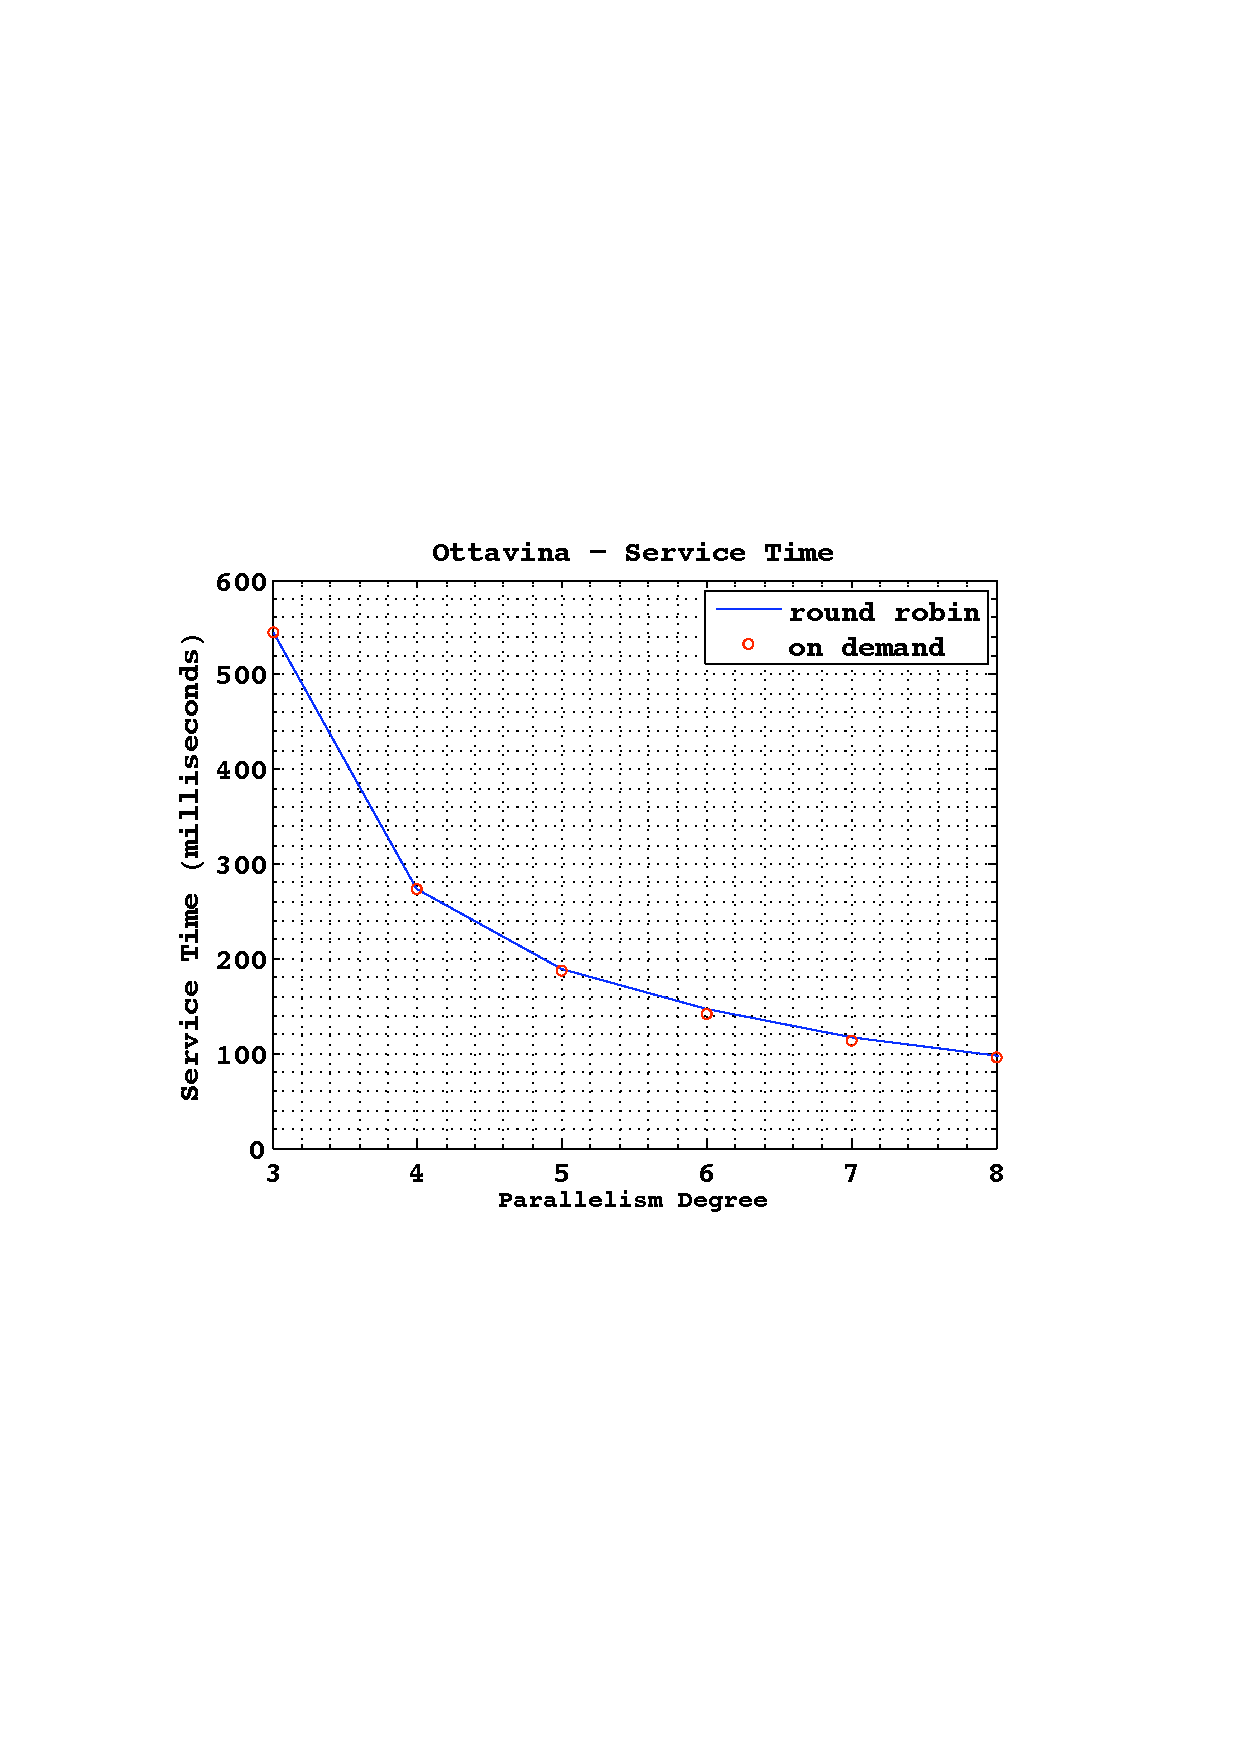
\includegraphics[width=\columnwidth,height=3.5in]{./CHART/ottavina_farm_1000_time}%
\label{graf:ottavina_farm_1000_time}}
\subfigure[]{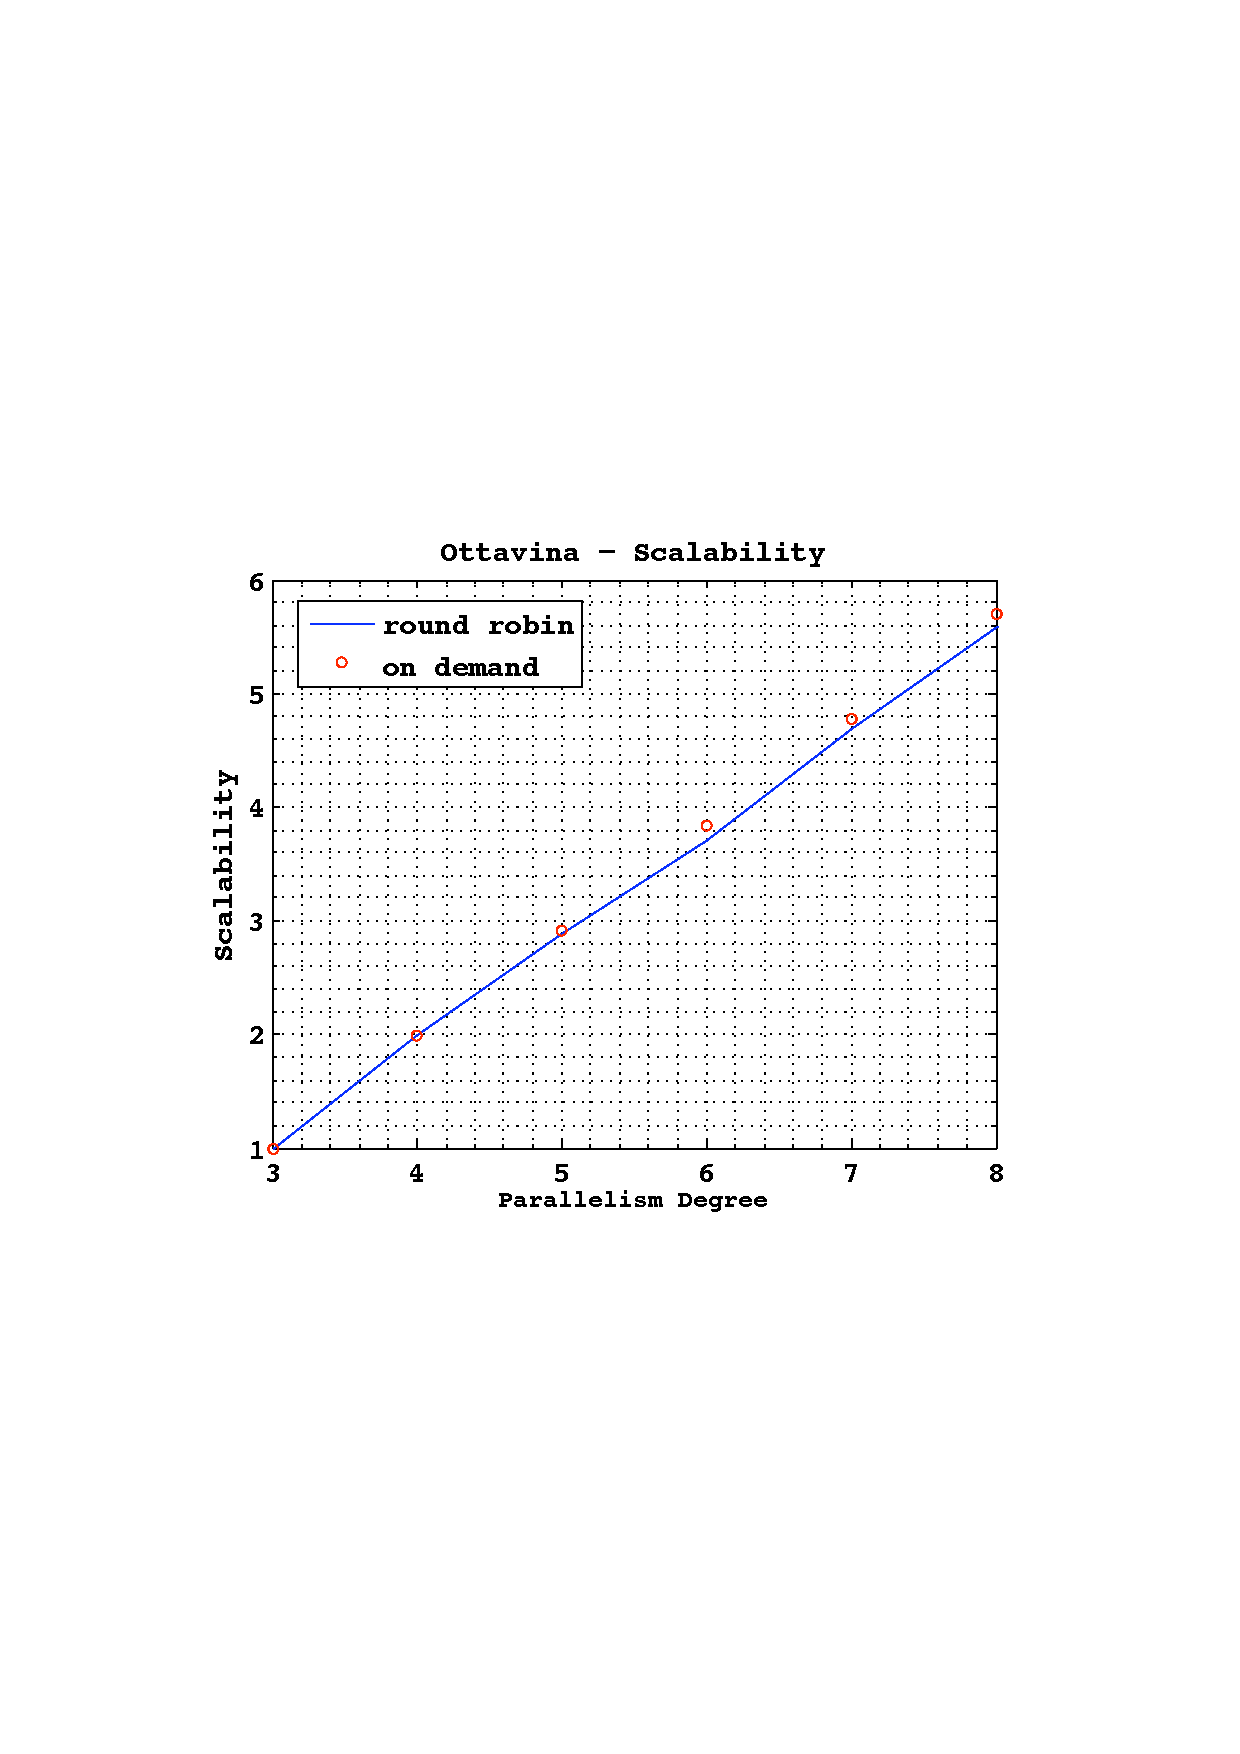
\includegraphics[width=\columnwidth,height=3.5in]{./CHART/ottavina_farm_1000_scala}%
\label{graf:ottavina_farm_1000_scala}}
\caption{ Service time of the farm implementation \ref{graf:ottavina_farm_1000_time} and relative scalability \ref{graf:ottavina_farm_1000_scala}. Test performed on Intel E5420 @ 2.50 GHz CPU with images of $10^6$ 8bit pixels. Parallelism degree is starting from 3 because of the service nodes (emitter and collector). }
\label{chart:ottavina_farm_1000}
\end{figure}

\begin{figure}[p]
\centering
\subfigure[]{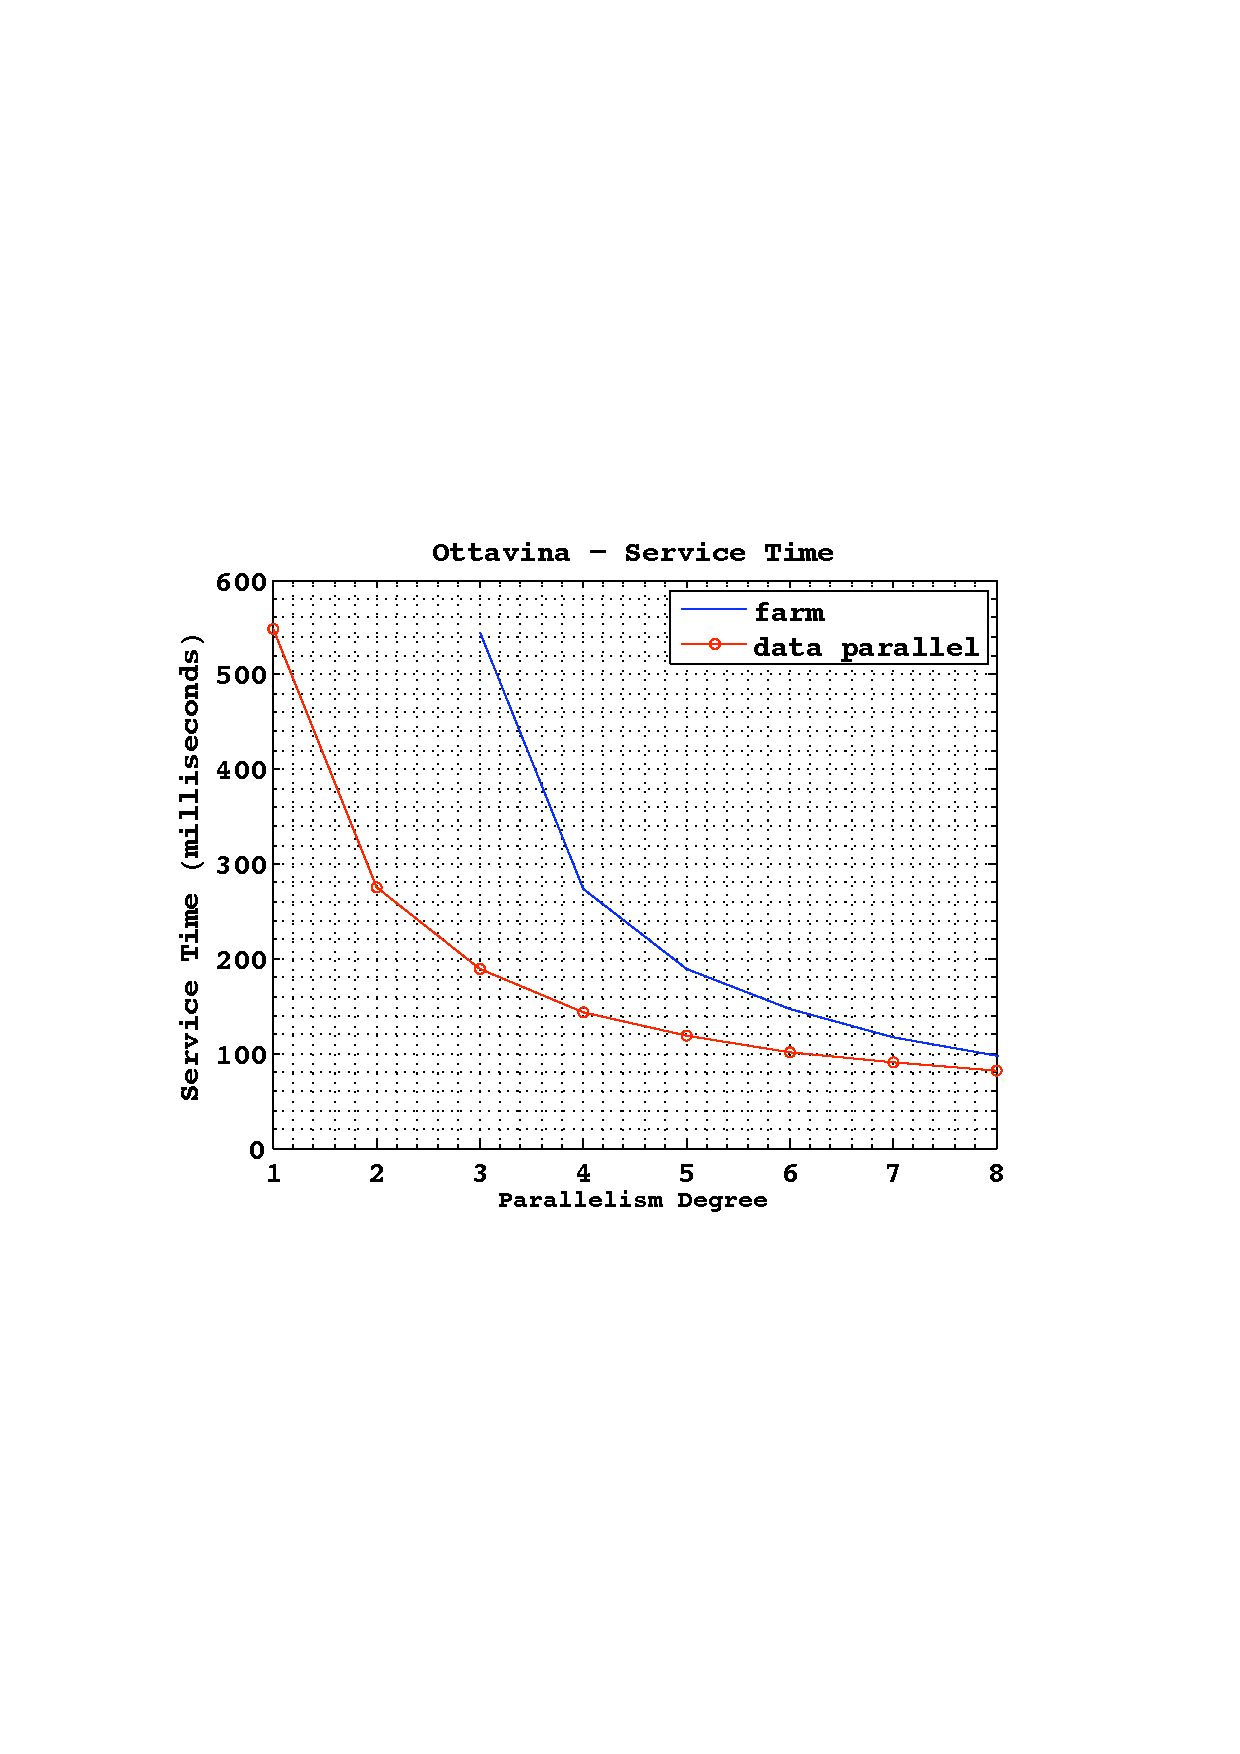
\includegraphics[width=\columnwidth,height=3.5in]{./CHART/ottavina_farmvsdata_1000_time}%
\label{graf:ottavina_data_1000_time}}
\subfigure[]{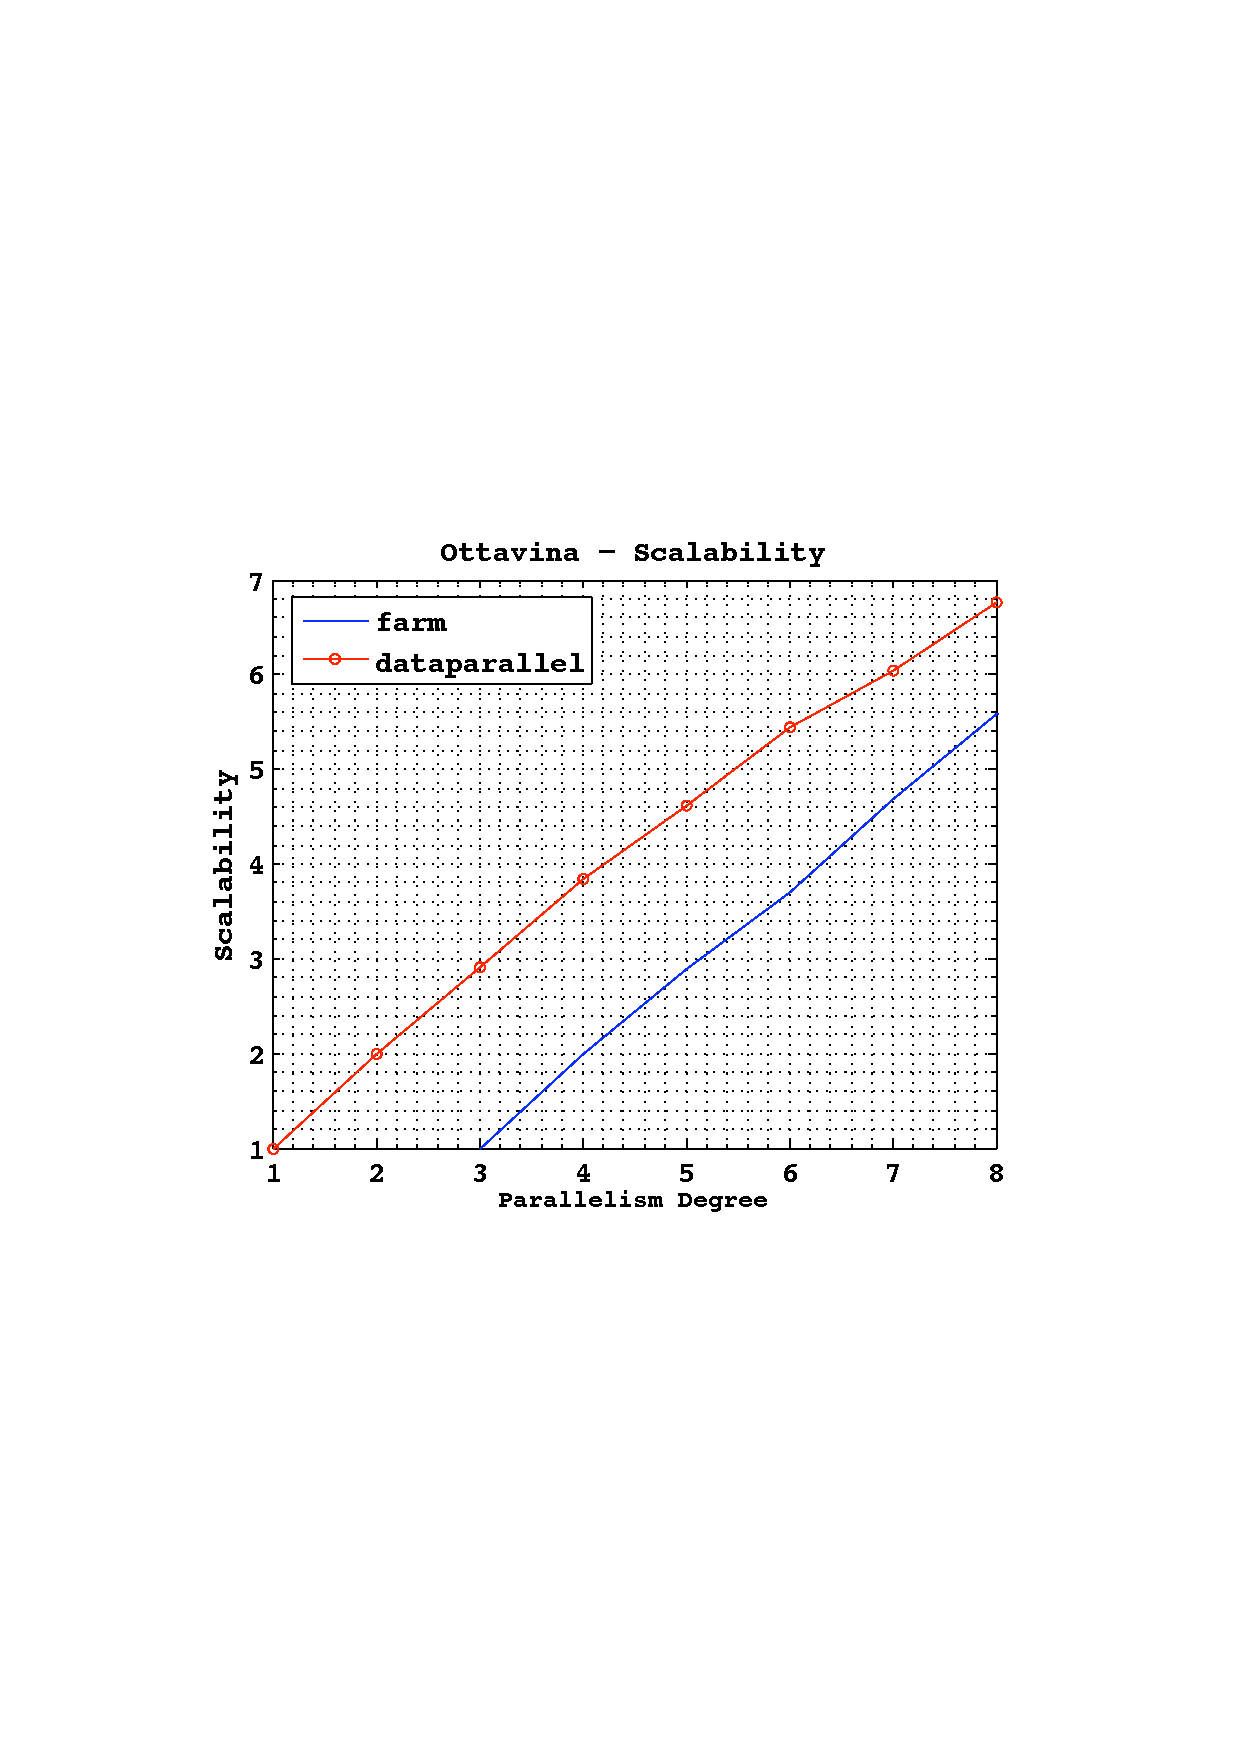
\includegraphics[width=\columnwidth,height=3.5in]{./CHART/ottavina_farmvsdata_1000_scala}%
\label{graf:ottavina_data_1000_scala}}
\caption{ Service time of the farm and data parallel implementation \ref{graf:ottavina_farm_1000_time} and relative scalability \ref{graf:ottavina_farm_1000_scala}. Test performed on Intel E5420 @ 2.50 GHz CPU with images of $10^6$ 8bit pixels.}
\label{chart:ottavina_data_1000}
\end{figure}

\begin{figure}[p]
\centering
\subfigure[]{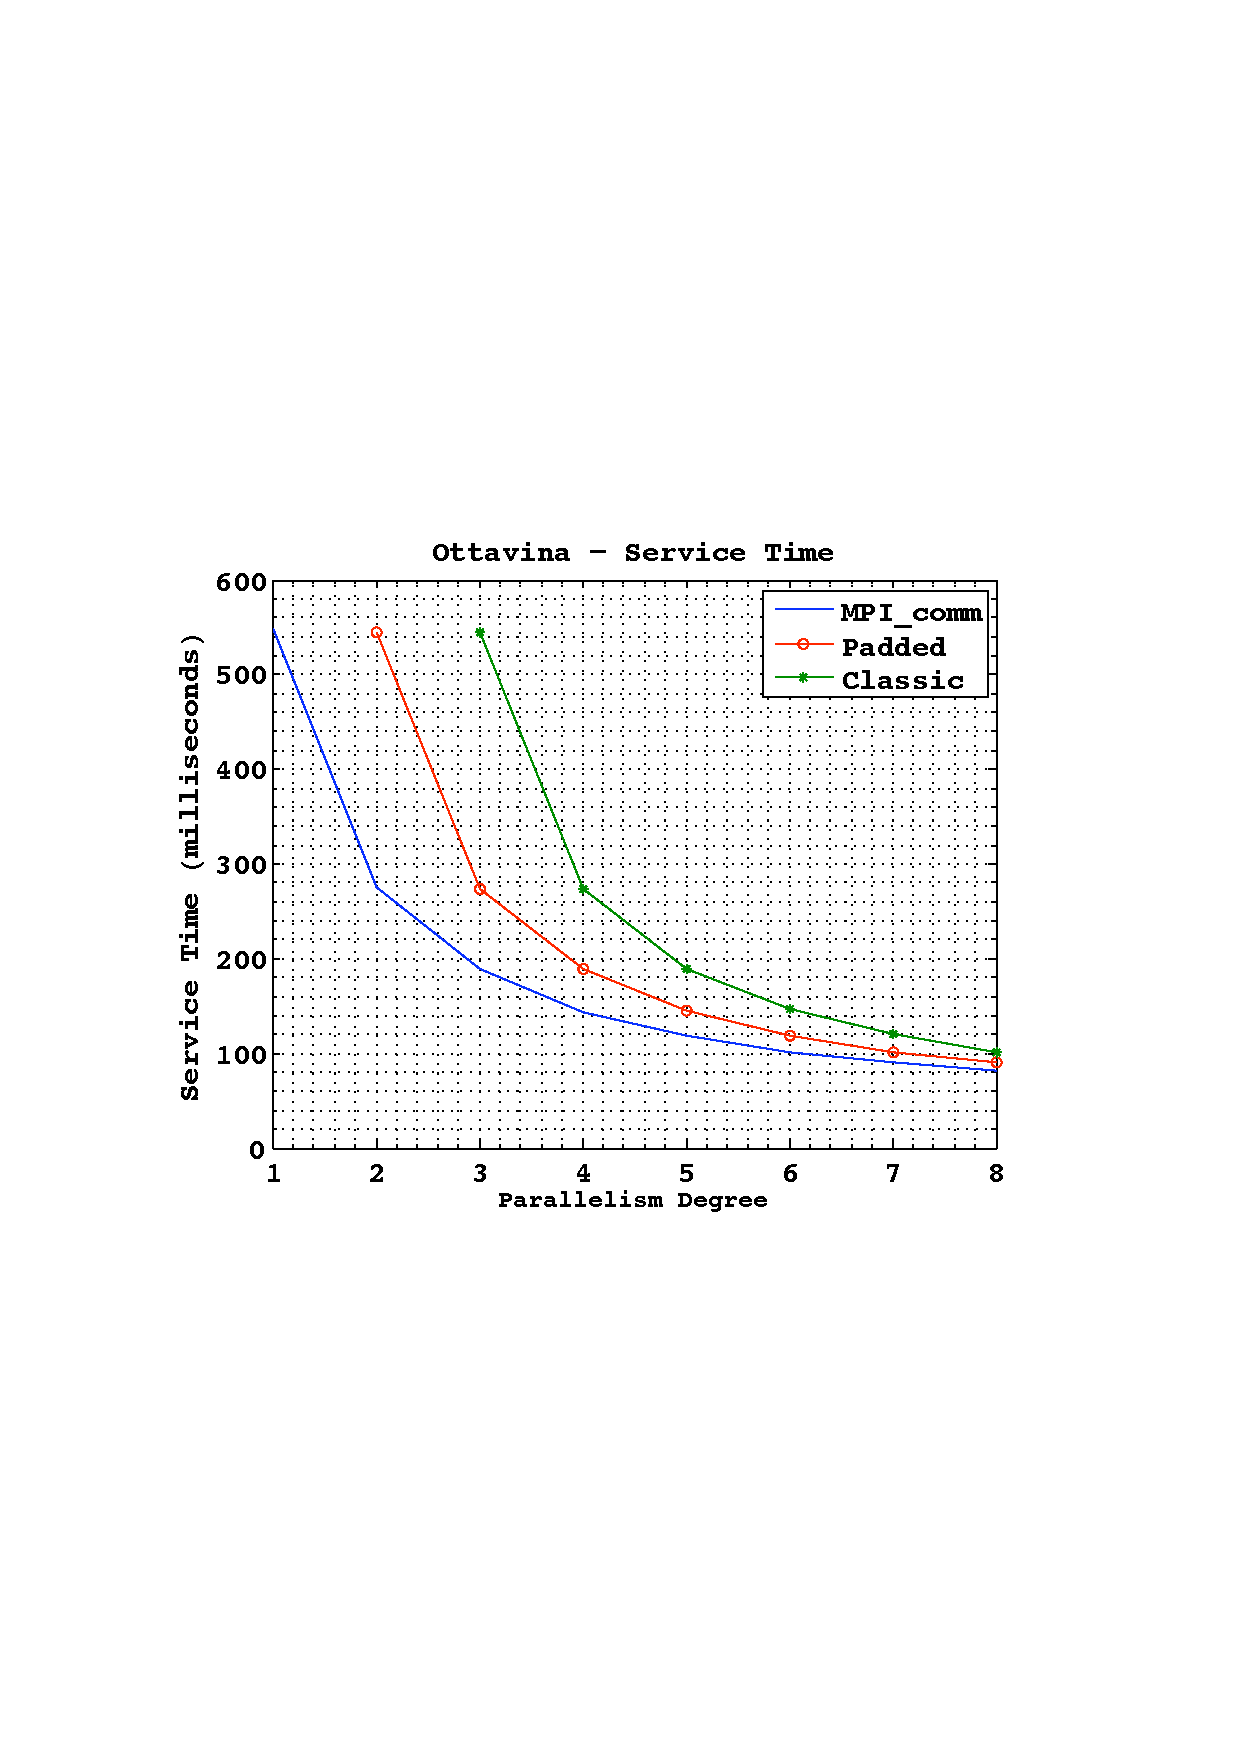
\includegraphics[width=\columnwidth,height=3.5in]{./CHART/ottavina_alldata_1000_time}%
\label{graf:ottavina_alldata_1000_time}}
\subfigure[]{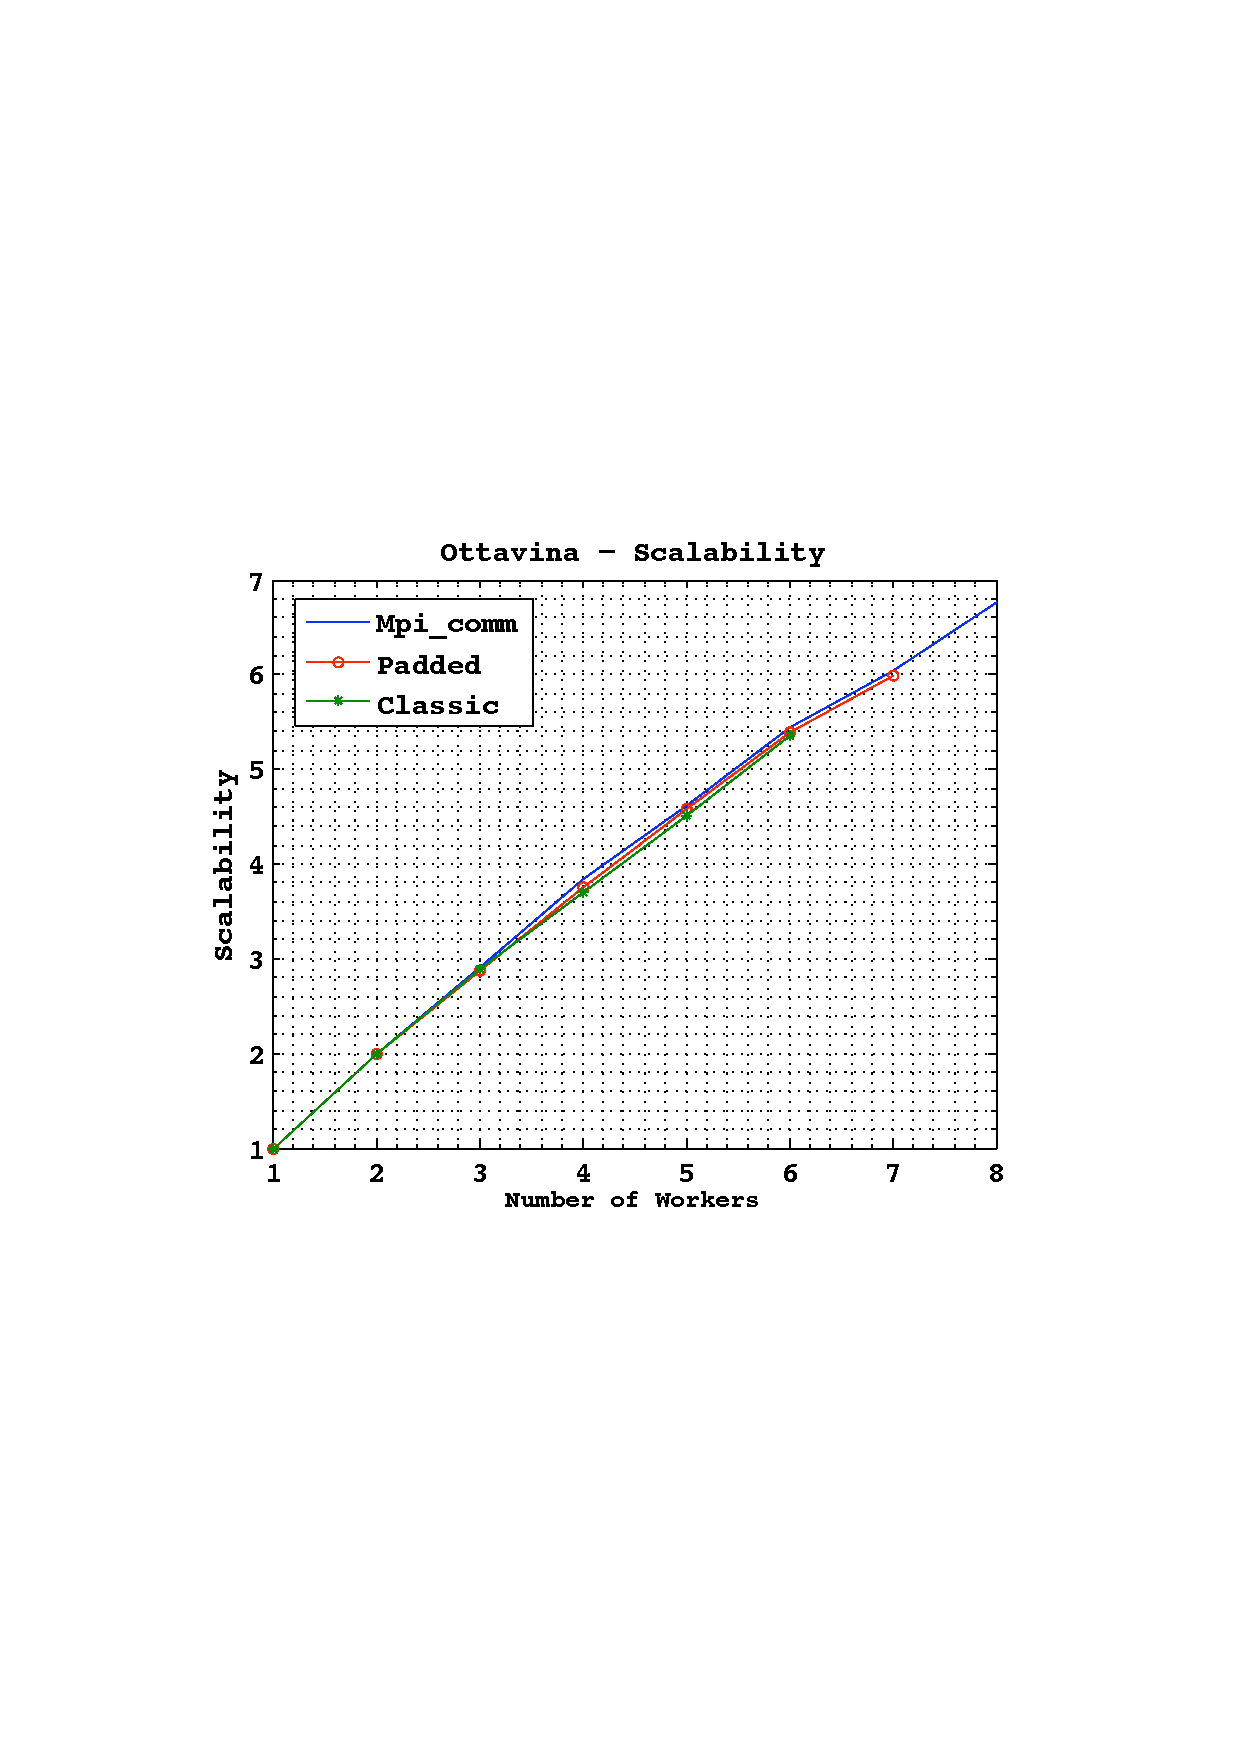
\includegraphics[width=\columnwidth,height=3.5in]{./CHART/ottavina_alldata_1000_scala}%
\label{graf:ottavina_alldata_1000_scala}}
\caption{ Service time of all the data parallel implementation \ref{graf:ottavina_farm_1000_time} and relative scalability, normalized with respect of the number of workers \ref{graf:ottavina_farm_1000_scala}. Test performed on Intel E5420 @ 2.50 GHz CPU with images of $10^6$ 8bit pixels.}
\label{chart:ottavina_alldata_1000}
\end{figure}

\begin{figure}[p]
\centering
\subfigure[]{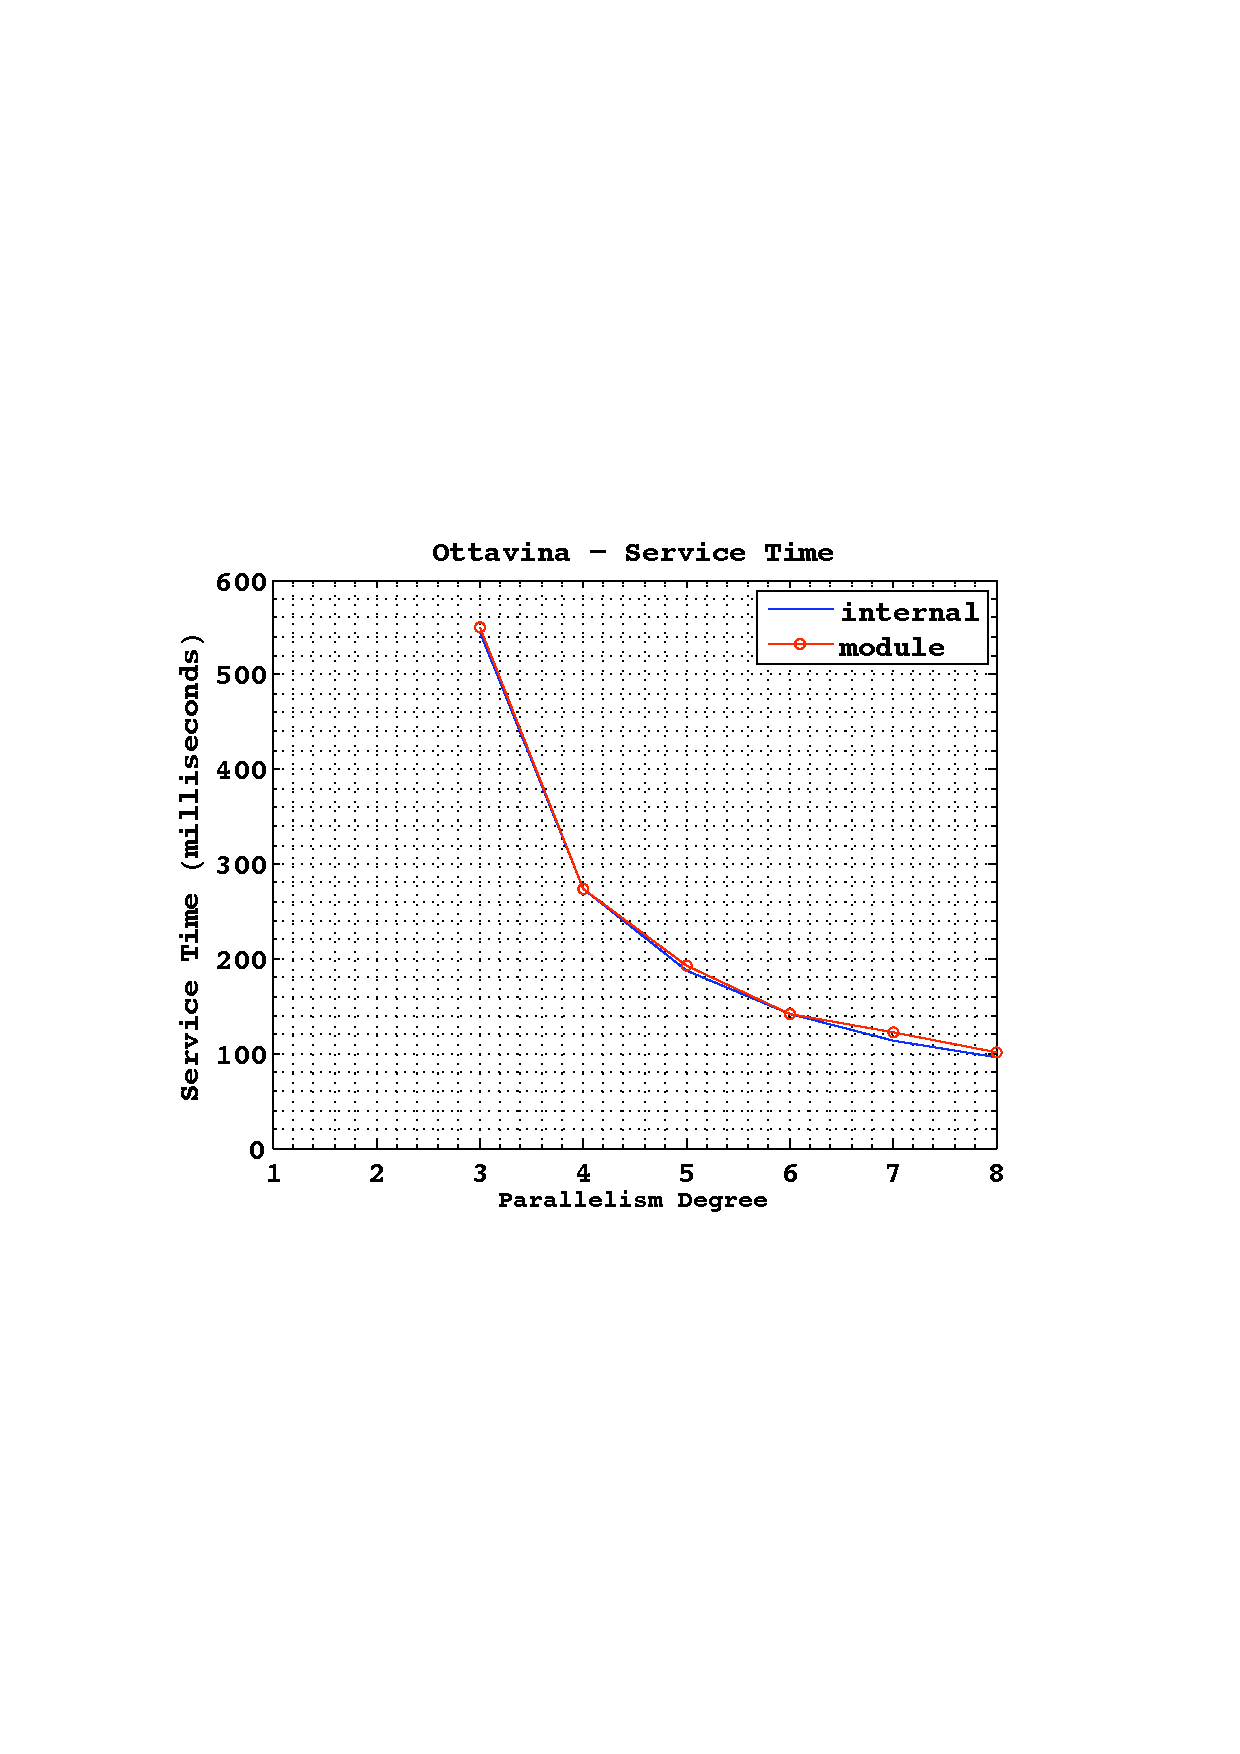
\includegraphics[width=\columnwidth,height=3.5in]{./CHART/farm_camera}%
\label{graf:farm_camera}}
\subfigure[]{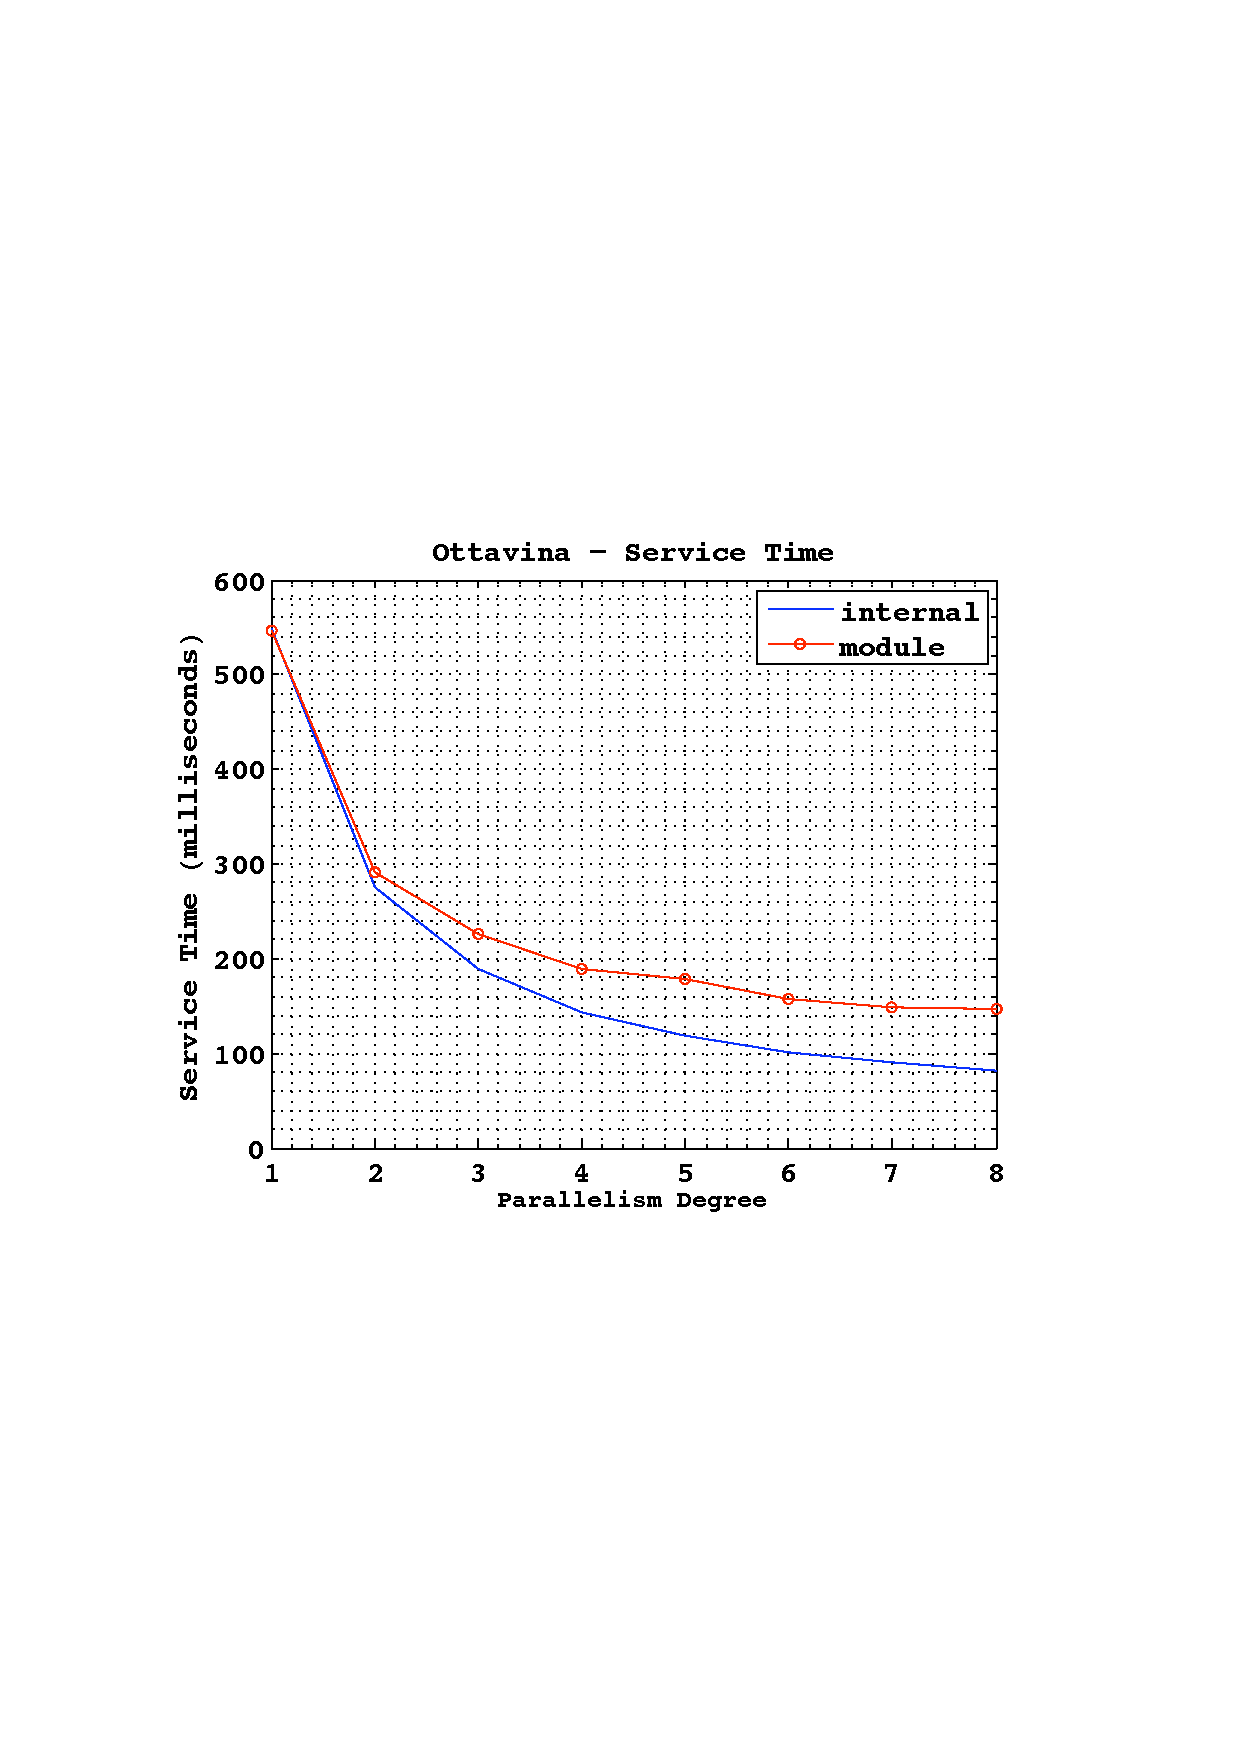
\includegraphics[width=\columnwidth,height=3.5in]{./CHART/data_camera}%
\label{graf:data_camera}}
\caption{ Comparison of application service time of farm implementation \ref{graf:ottavina_farm_1000_time} and data parallel implementation  \ref{graf:ottavina_farm_1000_scala} with or without external camera module. Test performed on Intel E5420 @ 2.50 GHz CPU with images of $10^6$ 8bit pixels.}
\label{chart:ottavina_camera}
\end{figure}

\begin{figure}[p]
\centering
\subfigure[]{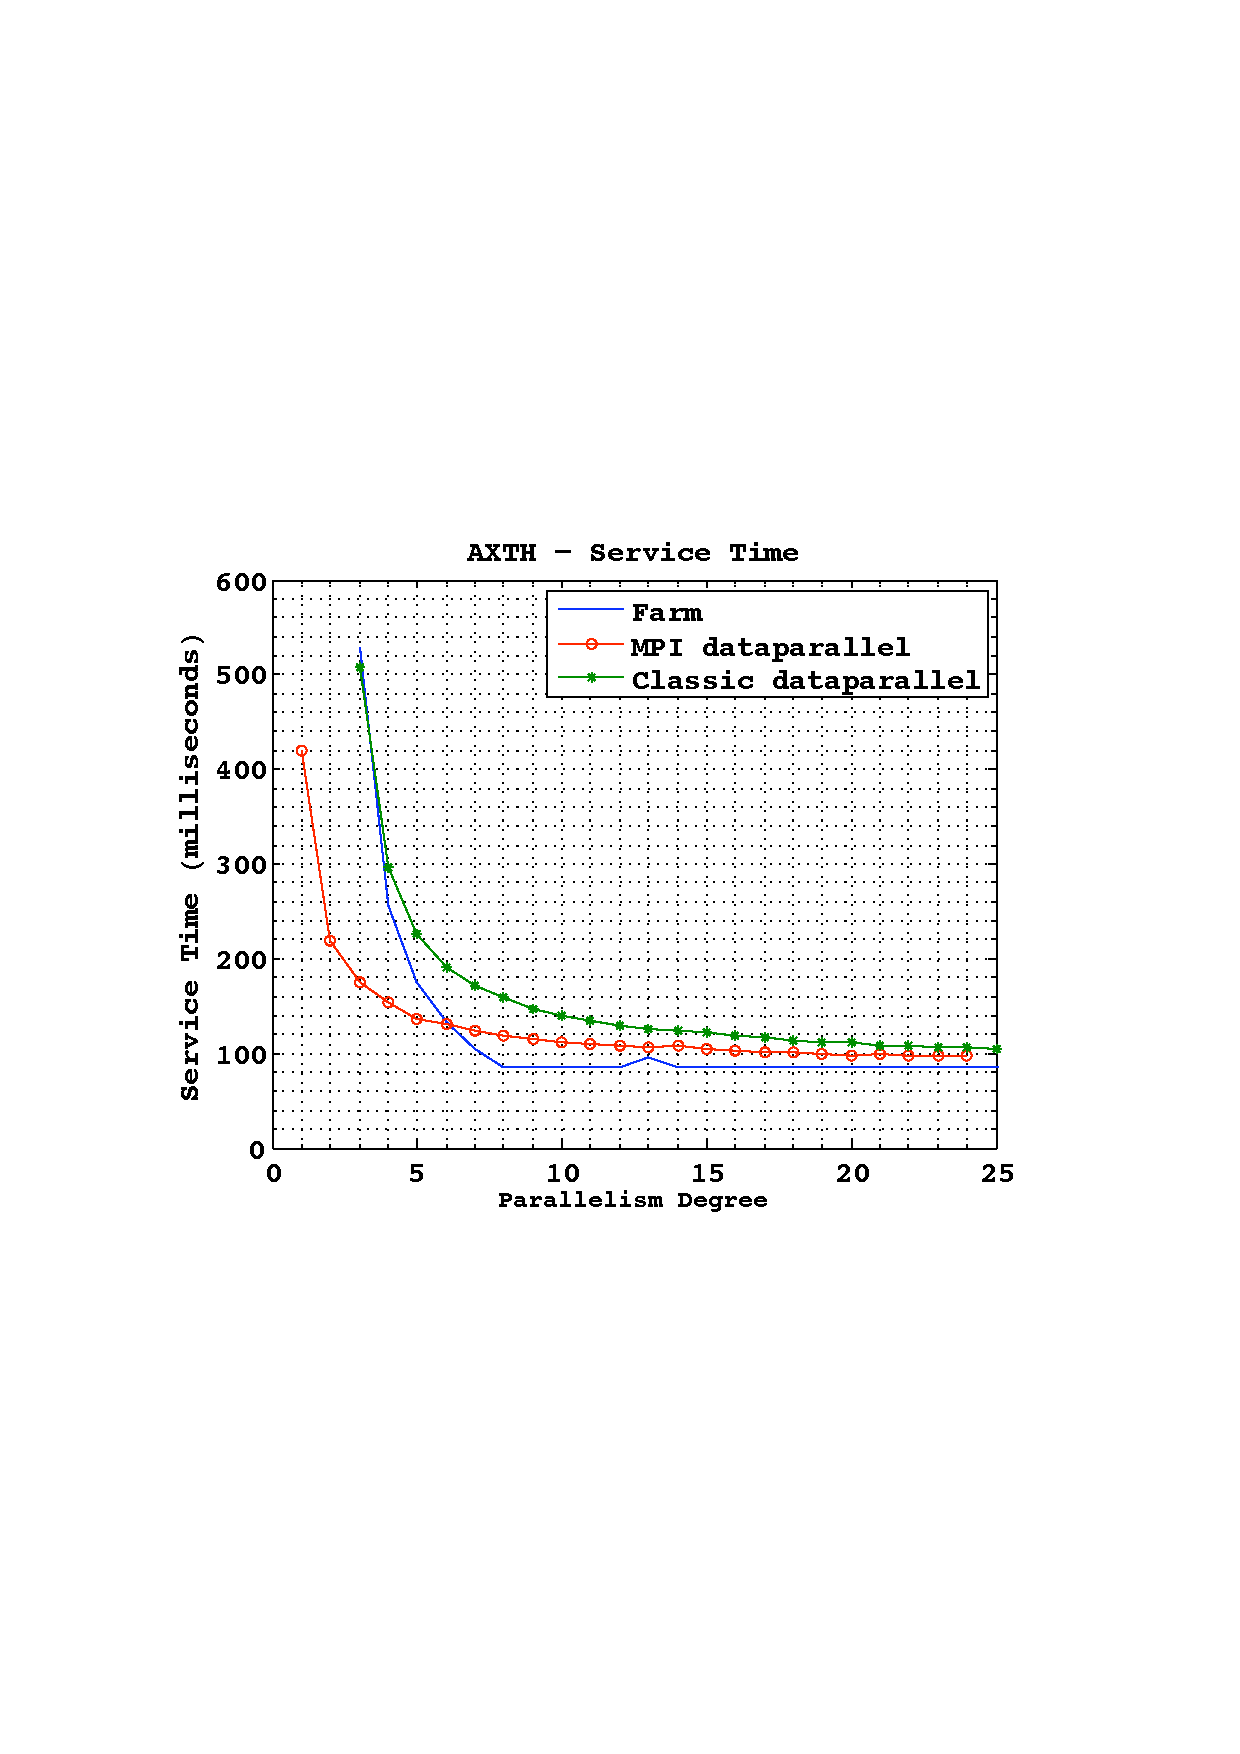
\includegraphics[width=\columnwidth,height=3.5in]{./CHART/axth_confronto_time}%
\label{graf:time_axth}}
\subfigure[]{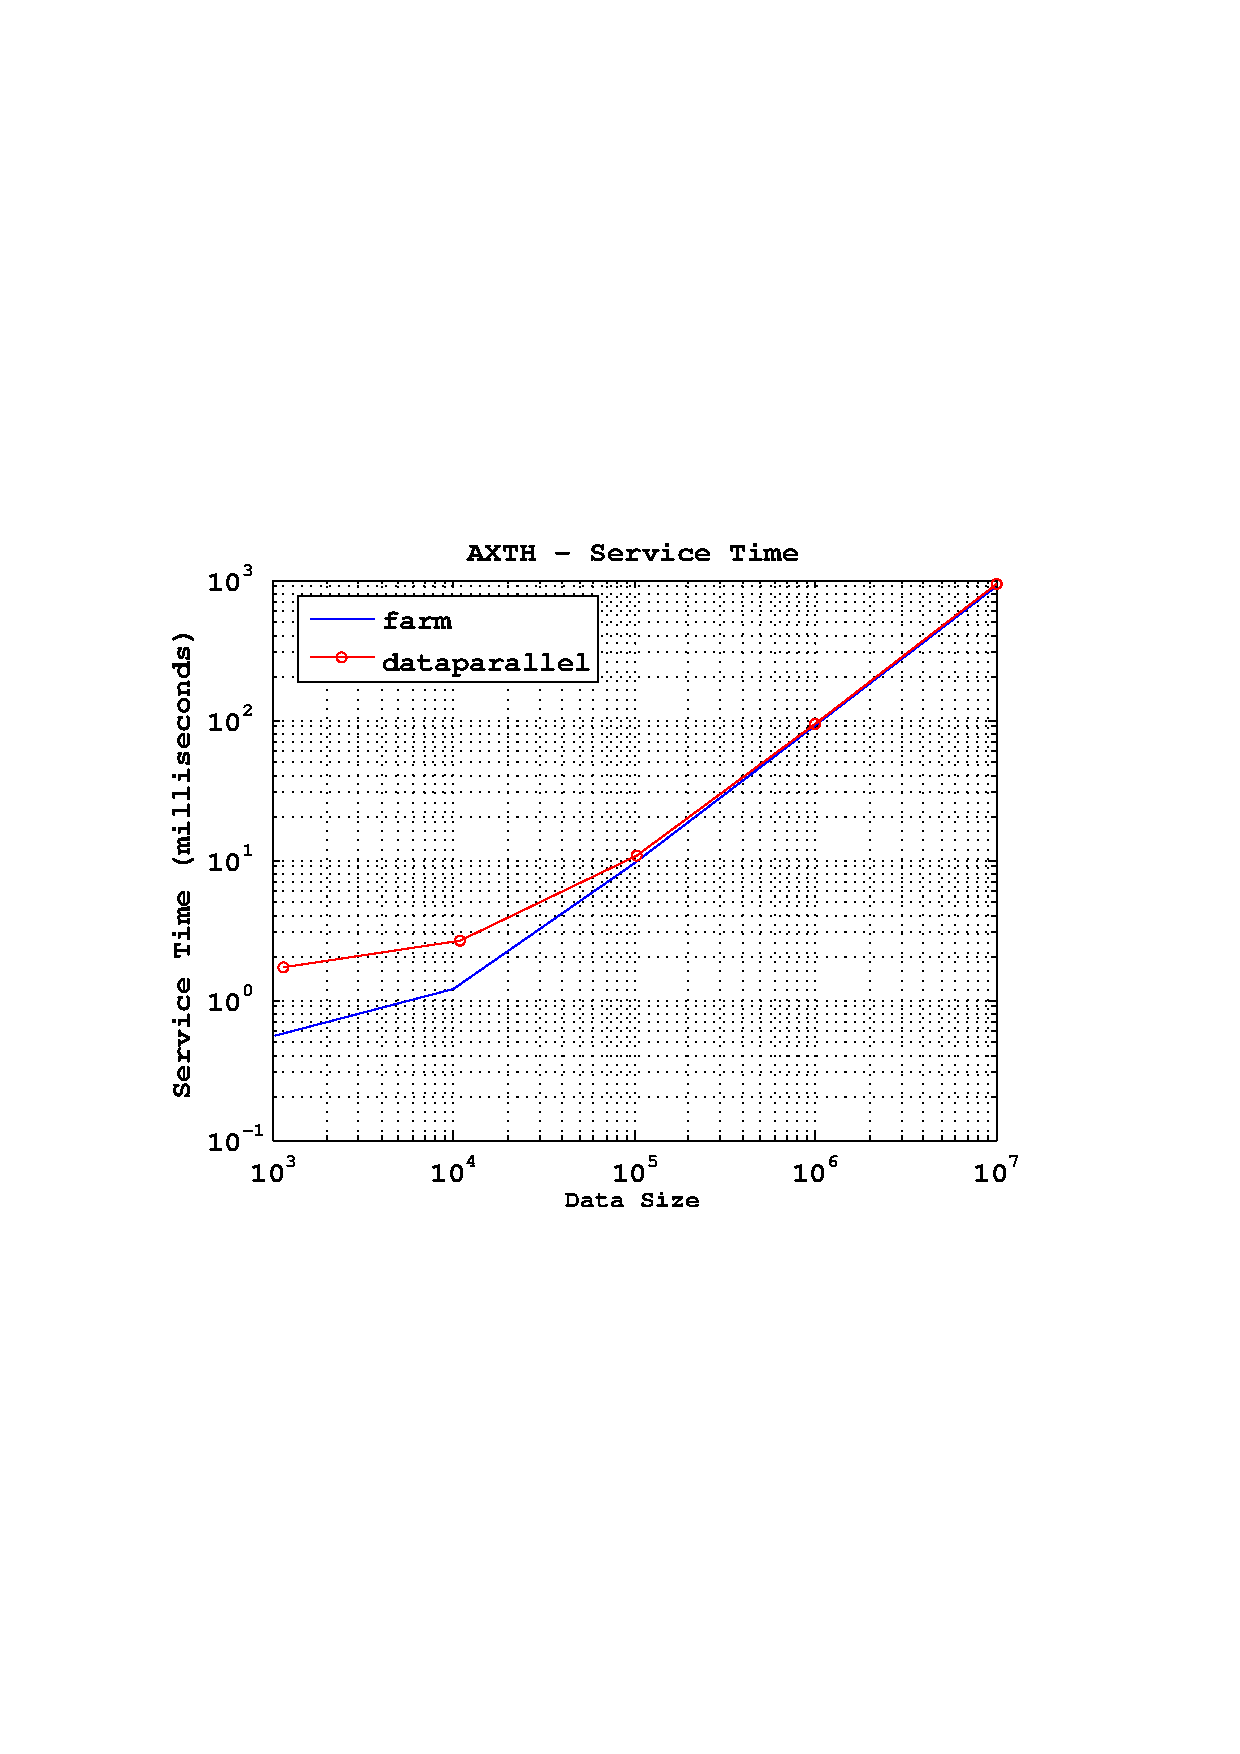
\includegraphics[width=\columnwidth,height=3.5in]{./CHART/axth_scalability}%
\label{graf:scala_axth}}
\caption{ Comparison of application service time of the various implementation \ref{graf:time_axth} and relative Scalability \ref{graf:scala_axth}. Test performed on a set of 20 nodes with Intel E7400 @ 2.80 GHz CPU. Images of $10^6$ 8bit pixels.}
\label{chart:axt}
\end{figure}

\begin{figure}[p]
\centering
\subfigure[]{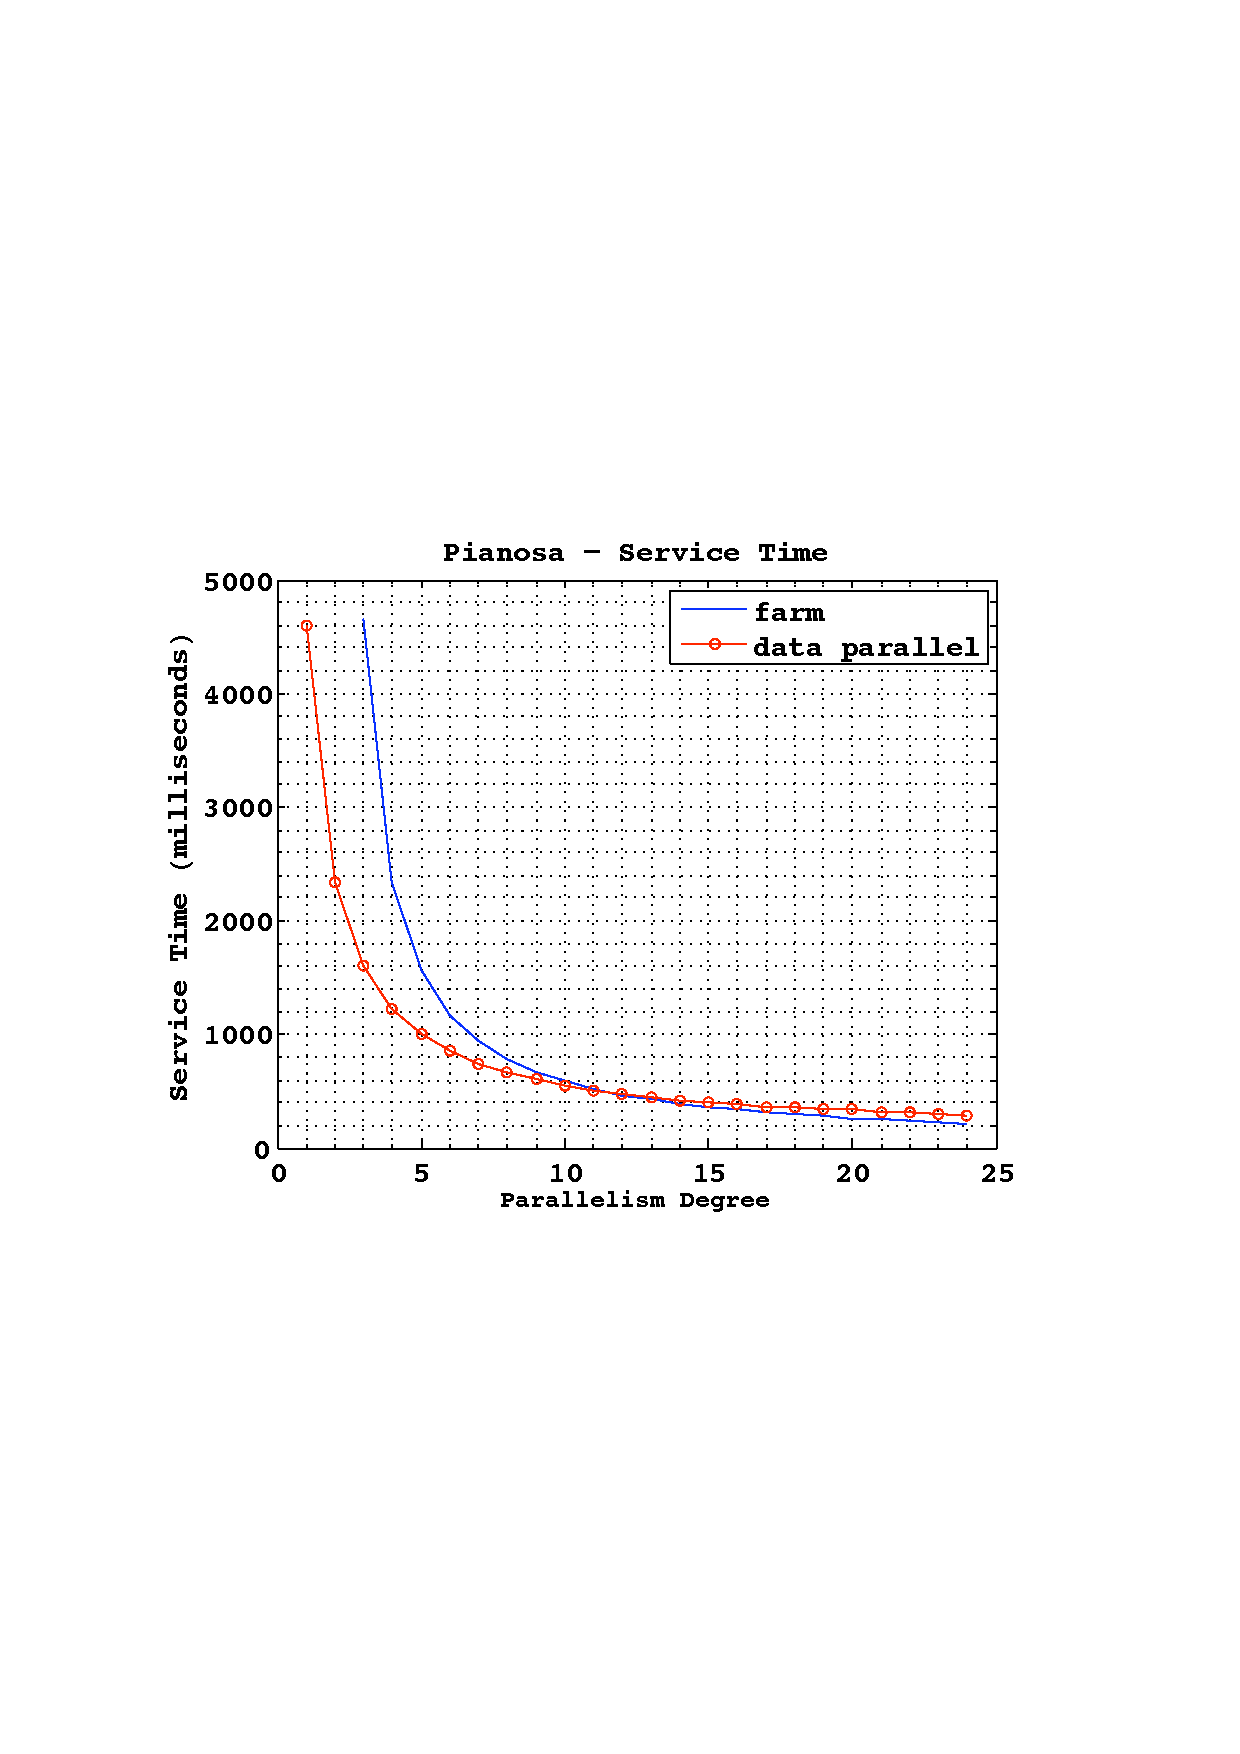
\includegraphics[width=\columnwidth,height=3.5in]{./CHART/pianosa_time3}%
\label{graf:pianosa_time}}
\subfigure[]{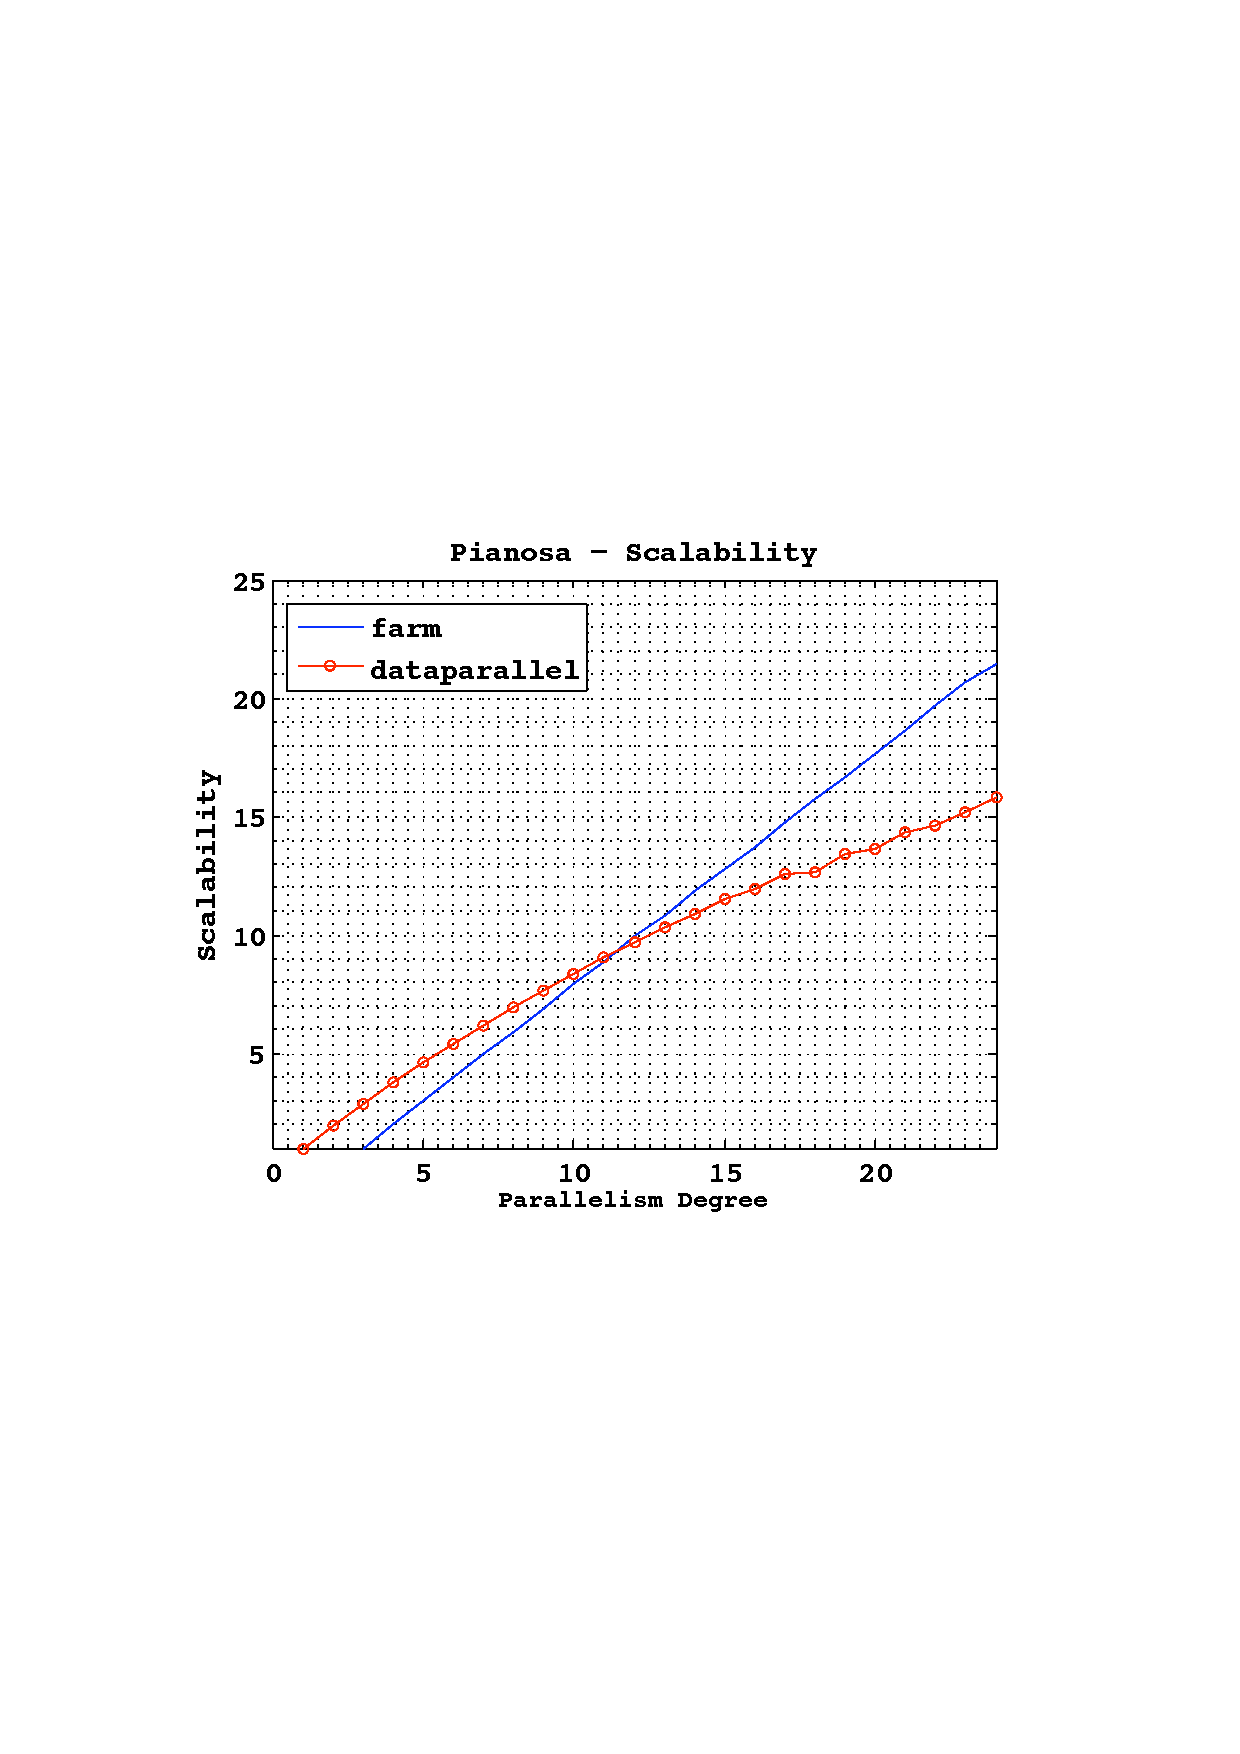
\includegraphics[width=\columnwidth,height=3.5in]{./CHART/pianosa_scala}%
\label{graf:pianosa_scala}}
\caption{ Service time on the Pianosa cluster of farm and data parallel implementation \ref{graf:time_axth} and relative scalability \ref{graf:pianosa_scala}.  Test is performed on a set of 24 nodes with Intel Pentium III @ 800 MHz CPU. Images of $10^6$ 8bit pixels.}
\label{chart:pianosa}
\end{figure}

\begin{figure}[p]
\centering
\subfigure[]{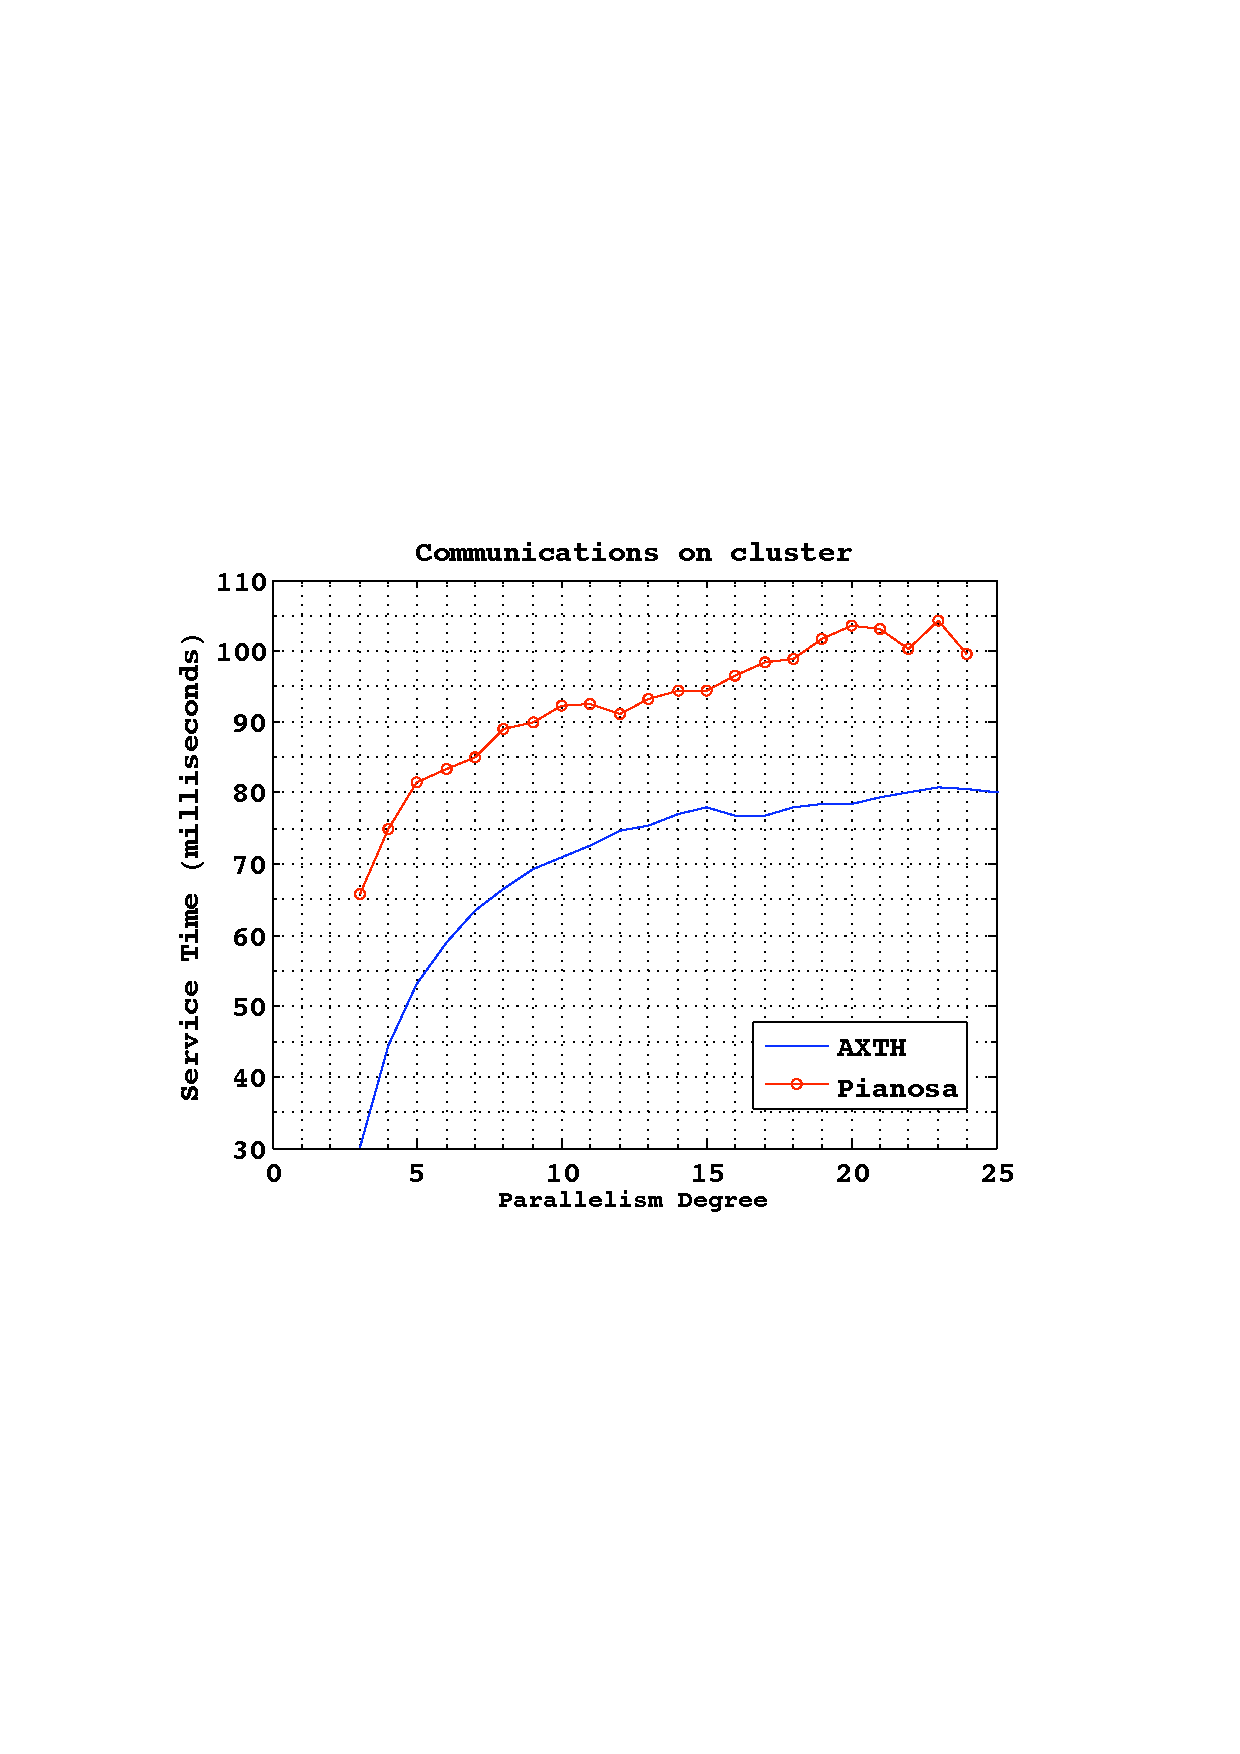
\includegraphics[width=\columnwidth,height=3.5in]{./CHART/Communication}%
\label{graf:communication}}
\subfigure[]{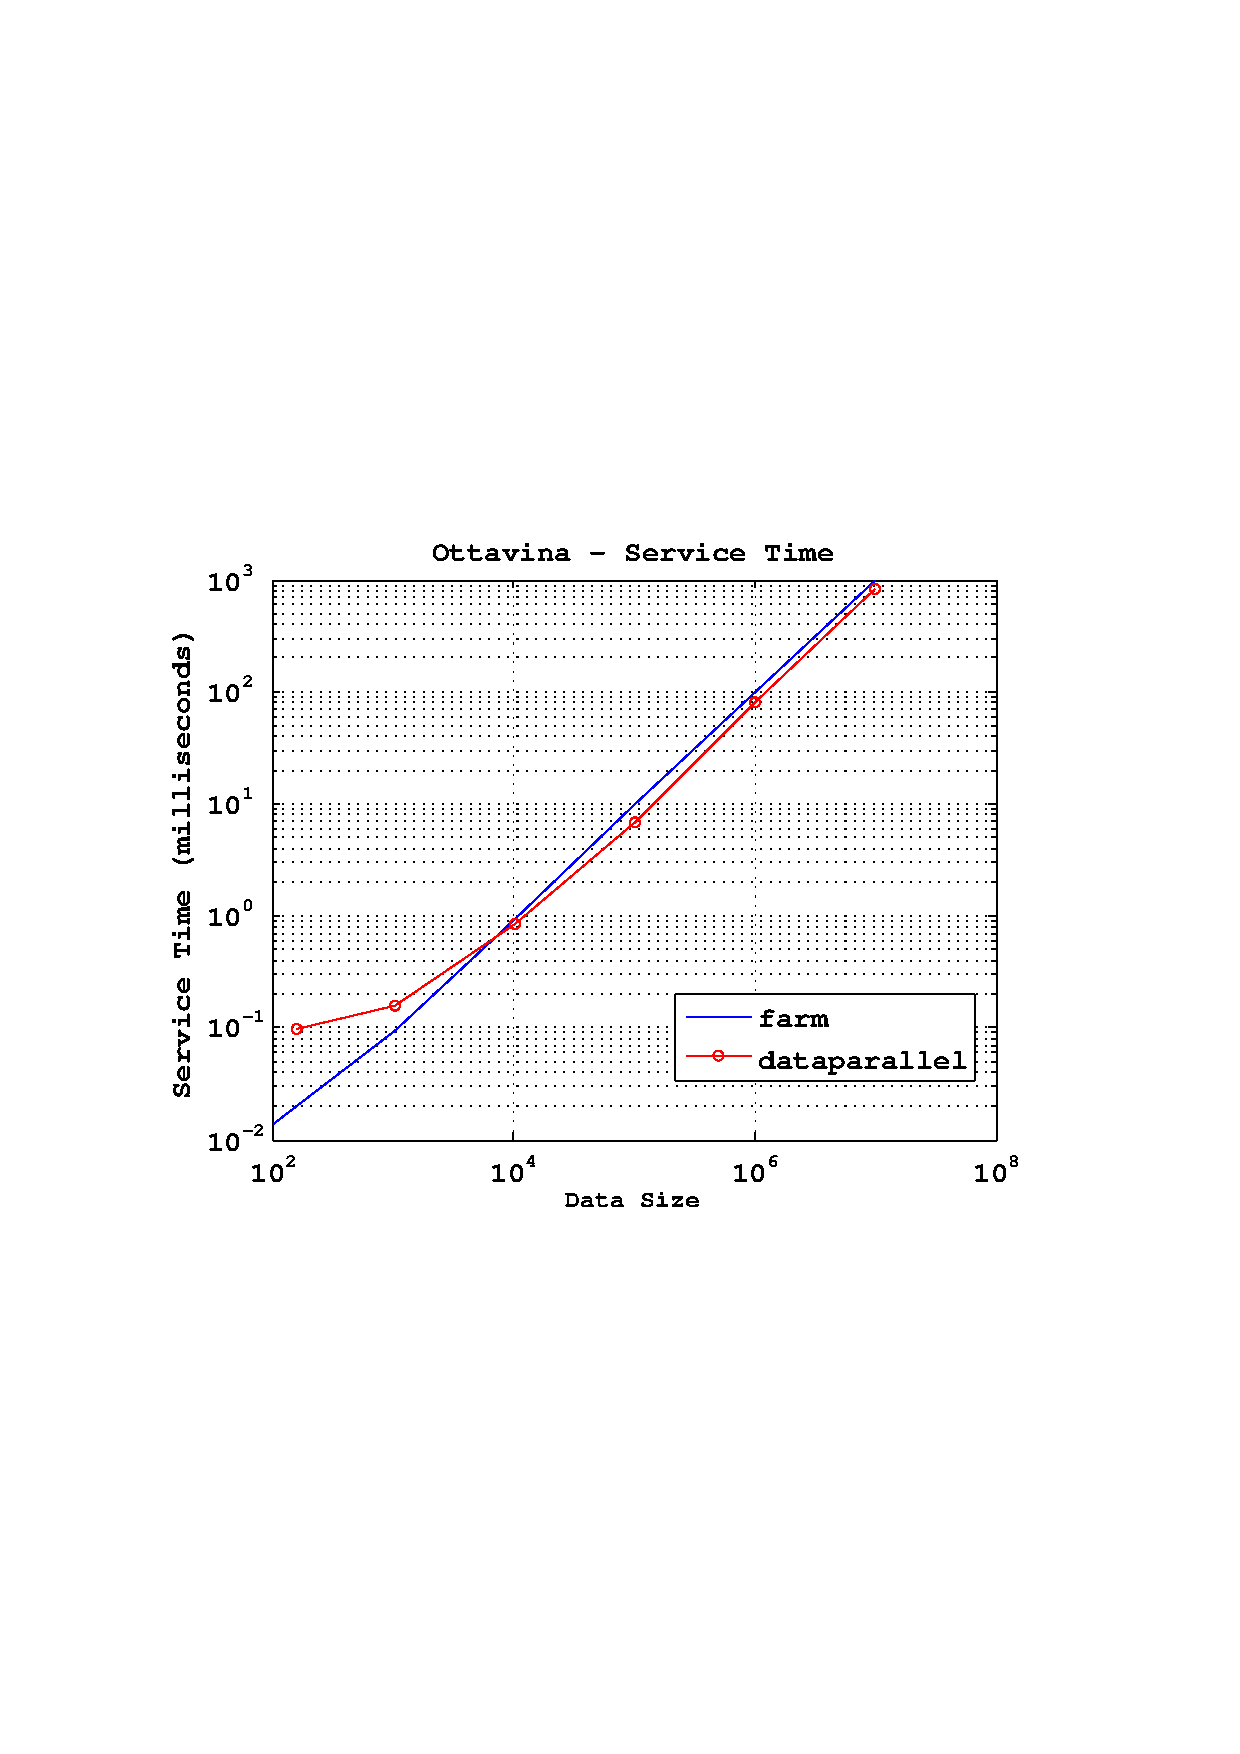
\includegraphics[width=\columnwidth,height=3.5in]{./CHART/ottavina_datascale}%
\label{graf:ottavina_datascale}}
\caption{ Communication time of the data parallel implementation, using MPI primitives on distributed memory architectures \ref{graf:communication}. Service time of the application executed on Ottavina varying the data set (dimension of the image) \ref{graf:ottavina_datascale}. }
\label{chart:ottavina_comm}
\end{figure}

\begin{figure}[p]
\centering
\subfigure[]{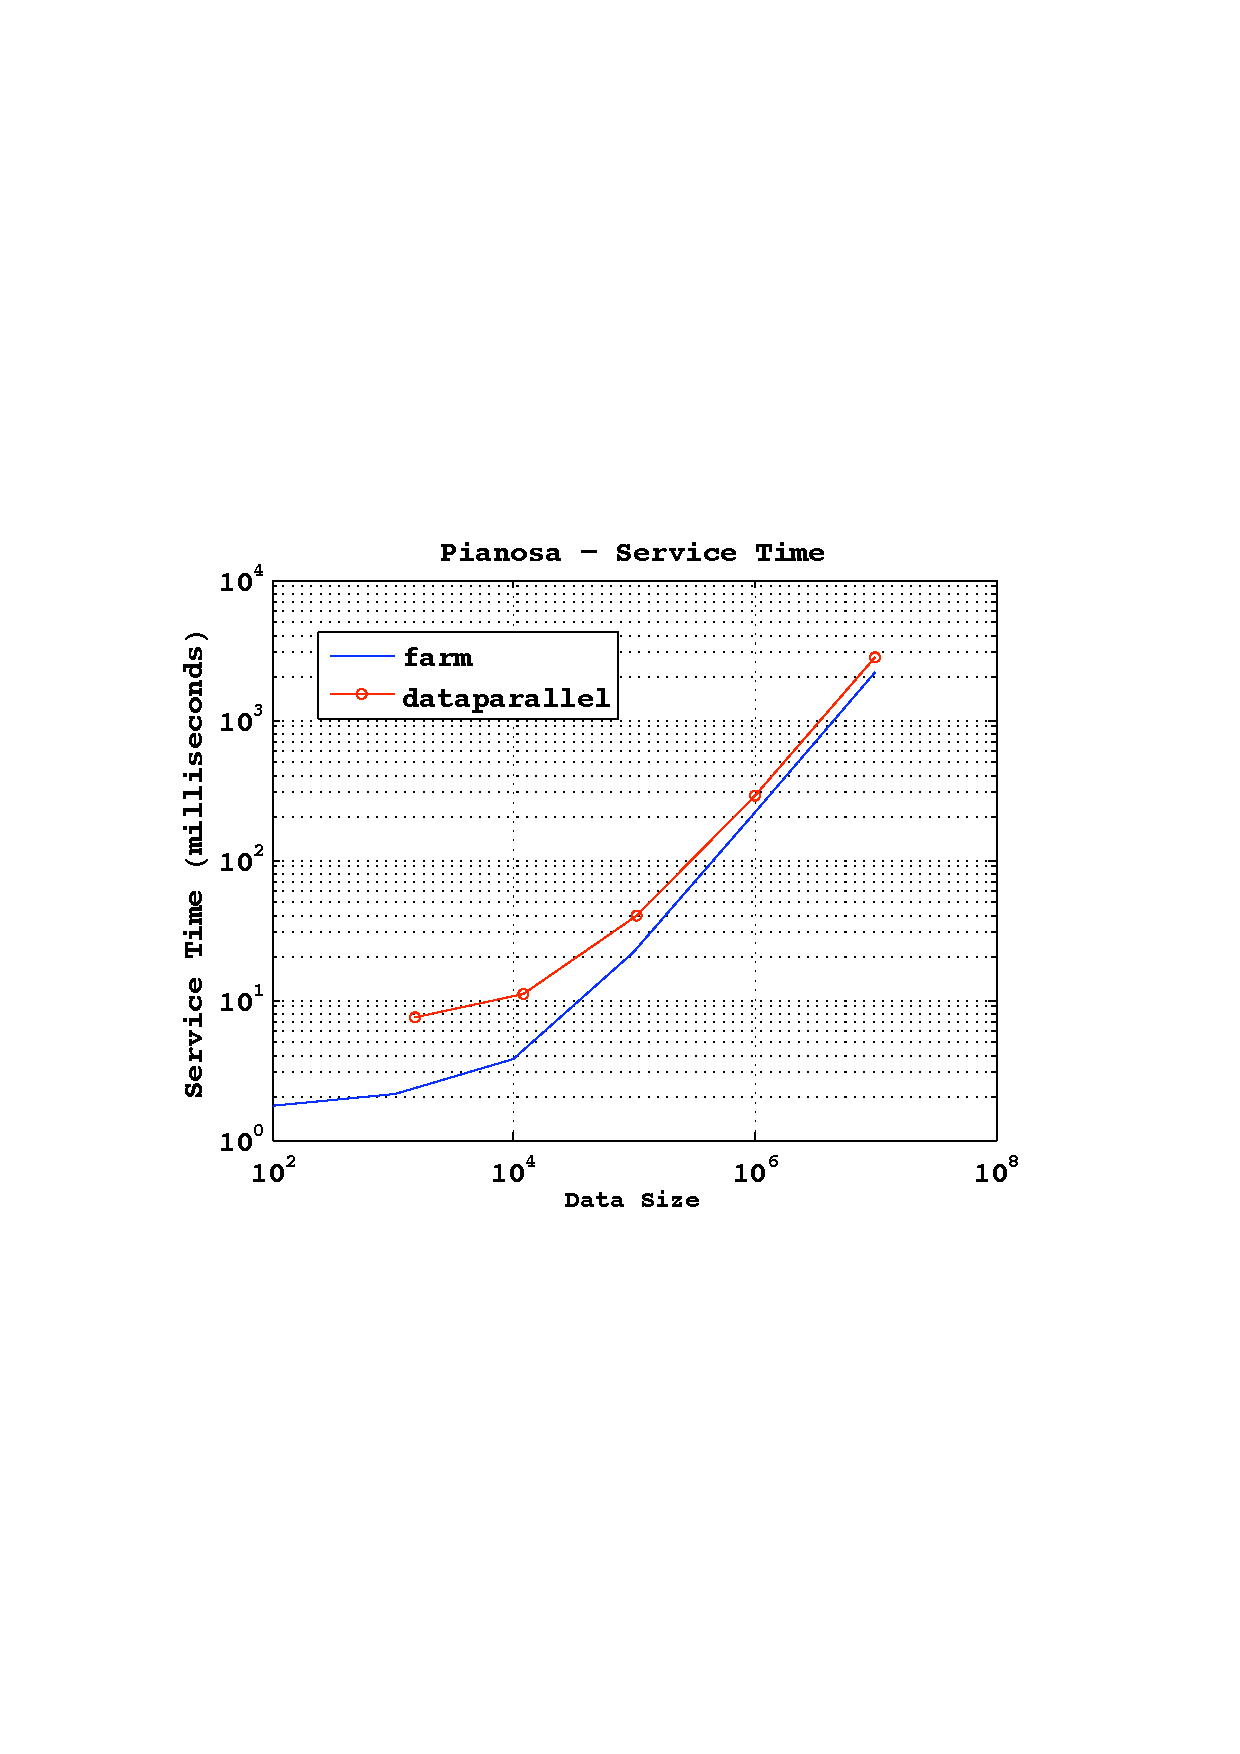
\includegraphics[width=\columnwidth,height=3.5in]{./CHART/pianosa_datascale}%
\label{graf:pianosa_datascale}}
\subfigure[]{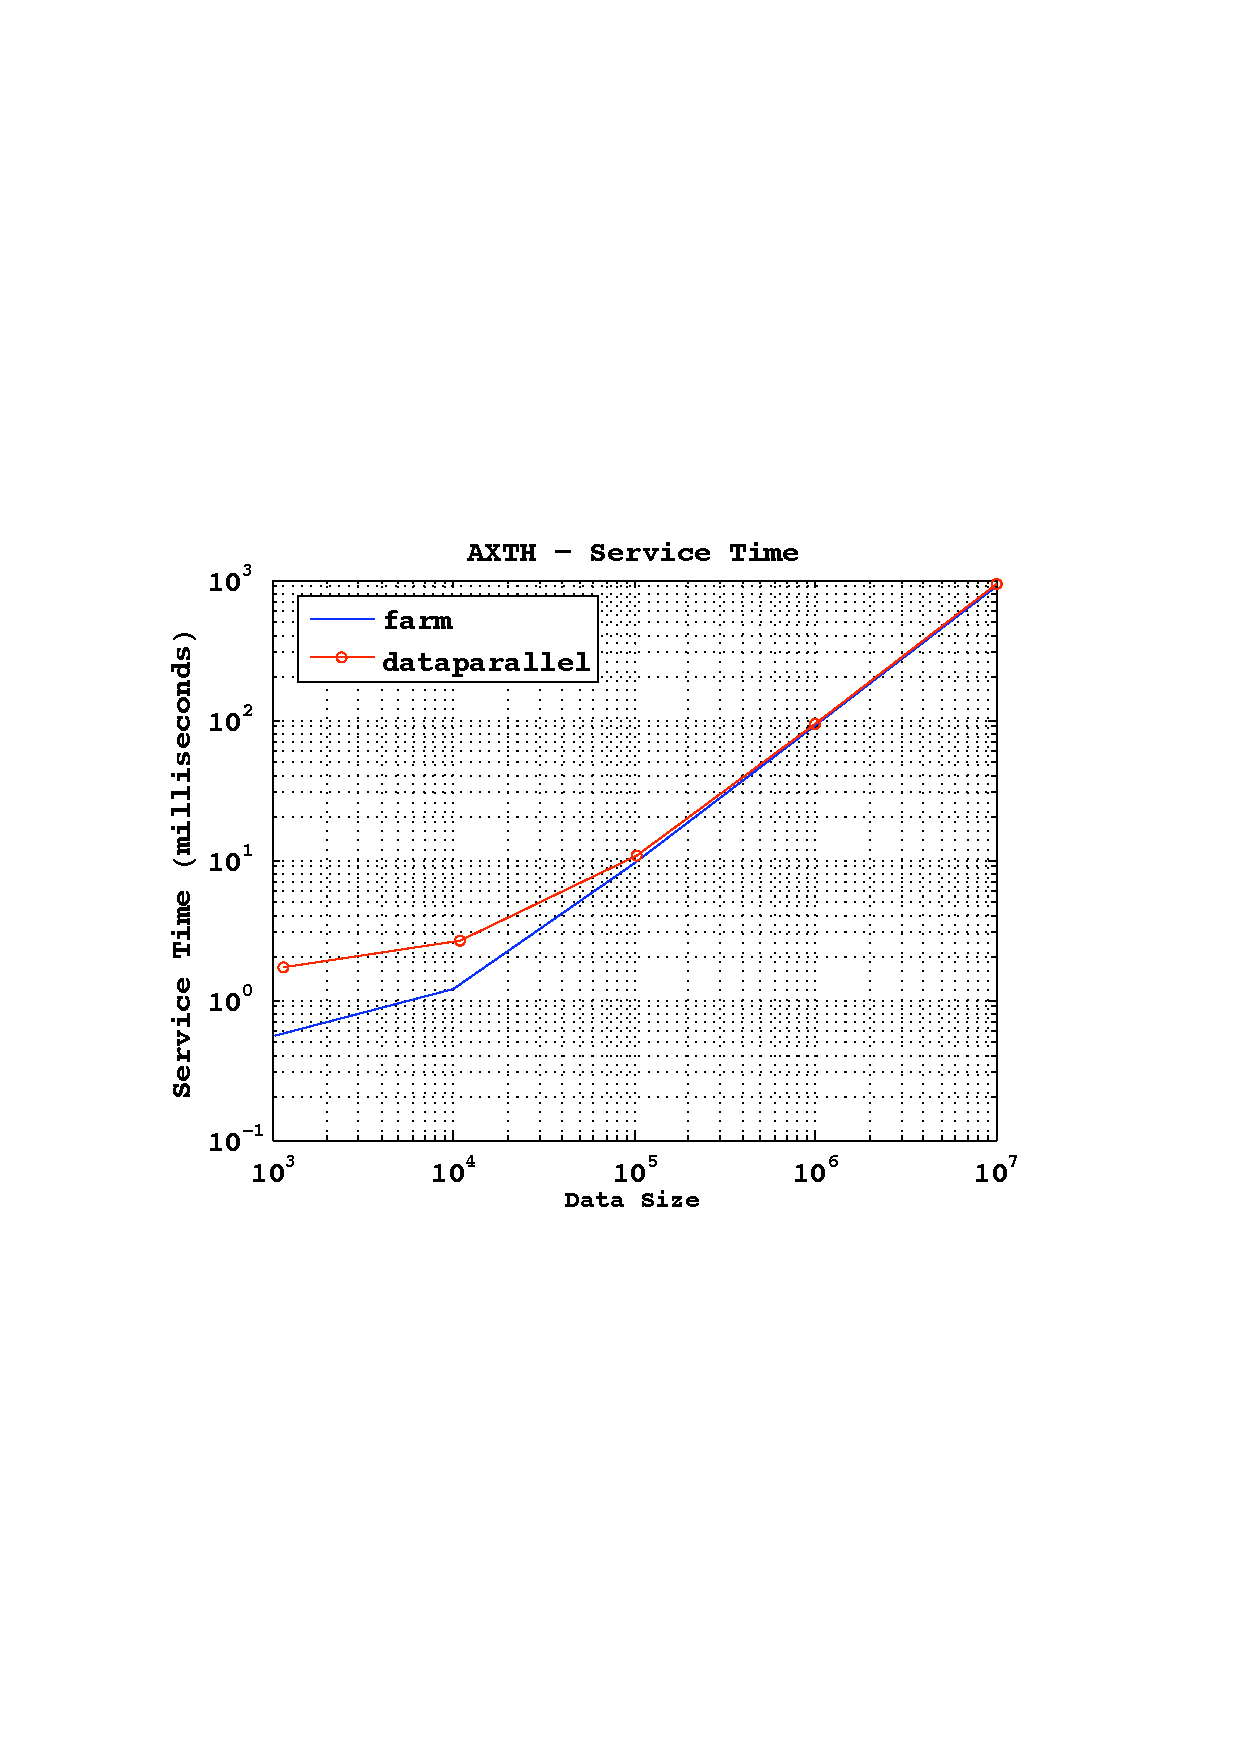
\includegraphics[width=\columnwidth,height=3.5in]{./CHART/axth_datascale}%
\label{graf:axth_datascale}}
\caption{ Service time of the application executed on Pianosa varying the data set (dimension of the image)  \ref{graf:pianosa_datascale}.
Service time of the application executed on Axth lab varying the data set (dimension of the image) \ref{graf:axth_datascale}. }
\label{chart:pianosa_axth}
\end{figure}
